\documentclass[a4paper]{article}

\usepackage[utf8]{inputenc}
\usepackage[T1]{fontenc}
\usepackage[italian]{babel}

\usepackage[margin=4.2cm, top=1.5cm, bottom=2.5cm]{geometry}

\usepackage{siunitx}
\usepackage{amsmath}
\usepackage{amssymb}
\usepackage{xfrac}
\usepackage{esint}
\usepackage[hidelinks]{hyperref}
\usepackage{graphicx}
\usepackage[font={sf}]{caption}
\usepackage{pdflscape}
\usepackage{makecell}
\usepackage{float}
\usepackage{subfig}
\usepackage{wasysym}
\usepackage{booktabs}
\usepackage{verbatim}

\setlength{\marginparwidth}{95pt}
\let\oldmarginpar\marginpar
\renewcommand\marginpar[1]{\oldmarginpar{\scriptsize\sffamily #1}}
\newcommand*\de{\mathrm{d}}
\newcommand*\pdv[2]{\frac{\partial #1}{\partial #2}}
\newcommand*\dv[2]{\frac{\de #1}{\de #2}}
\DeclareMathOperator\Ei{Ei}
\newcommand*\is{\equiv}
\newcommand\cs{\ensuremath{^{\text{137}}\text{Cs}}}
\newcommand\co{\ensuremath{^{\text{60}}\text{Co}}}
\newcommand\na{\ensuremath{^{\text{22}}\text{Na}}}
\newcommand\am{$^{\text{241}}\text{Am}$}
\newcommand\sr{$^{\text{90}}\text{Sr}$}

\sisetup{%
separate-uncertainty=true,
multi-part-units=single,
exponent-product=\cdot}

\frenchspacing

\title{Relazione di laboratorio:\\
Esperienza 4: Annichilazione del positrone}
\author{Andrea Marasciulli
\and Giacomo Petrillo
\and Roberto Ribatti}
\date{24 aprile -- 25 maggio 2018}

\begin{document}

\maketitle

\begin{abstract}

Misuriamo la massa dell'elettrone con una precisione maggiore dell'$1\permil$ facendo felice Punzi e (forse) il rate di cattura elettronica. Se siamo fortunati vediamo anche il positronio decadere in 3 fotoni.

\end{abstract}

{\tableofcontents}

\newpage
\section{Introduzione}

L'obiettivo principale dell'esperienza è la misura della massa del positrone sfruttando il decadimento $\beta^+$ del \na{}. Poi misuriamo l'efficienza dei rivelatori per stimare il rate di cattura elettronica rispetto al decadimento $\beta^+$. Infine cerchiamo di provare l'esistenza dell'annichilazione i 3 fotoni.
\subsection{Obiettivo}

Verificare l'andamento della sezione d'urto differenziale Rutherford per angoli acuti,
verificare la presenza di backscattering,
studiare la perdita di energia,
verificare il rapporto delle cariche nucleari di oro e alluminio.


\section{Teoria}

\subsection{Spettro delle sorgenti a disposizione}

La nostra sorgente di \na{} ha 3 modi di decadimento:
\begin{itemize}
\item decadimento $\beta^+$ con $E_e=\SI{545}{keV}$, BR=90.4\%;
\item cattura elettronica (BR=9.5\% ) con la conseguente emissione di un fotone di energia \SI{1274}{keV} da parte del $^{22}$Ne formatosi;
\item decadimento $\beta^-$ con BR=0.1\%.
\end{itemize}

Useremo i decadimenti $\gamma$ del \cs{} (\SI{662}{keV}) e del \co{} (\SI{1173}{keV}, \SI{1332}{keV}) per calibrare il nostro apparato.

\marginpar{Scrivere perché non usiamo l'americio?}

\subsection{Fenomenologia dei rivelatori}

\marginpar{Scrivere materiale e dimensioni nella sezione ``apparato''}

Nel range di energie dei fotoni in cui lavoriamo, i processi di diffusione possibili sono gli scattering Rayleigh e Compton e l'effetto fotoelettrico.
Lo scattering Rayleigh, in quanto completamente elastico, non rilascia energia nel calorimetro.
Nella diffusione Compton il fotone cede una parte dell'energia ad un elettrone del nostro calorimetro e possiamo misurare l'energia persa da quest'ultimo. L'energia persa dal fotone segue la distribuzione di Klein-Nishina.
\marginpar{Klein-Nishina è la distribuzione angolare, non dell'energia.}
Se il fotone esegue un effetto fotoelettrico, perde tutta la sua energia cedendola ad un elettrone ed è l'unico modo che abbiamo per conoscere l'energia del fotone incidente.

A questo quadro si possono aggiungere processi di ordine superiore, come un numero maggiore di rimbalzi Compton all'interno del cristallo oppure un effetto fotoelettrico eseguito dopo uno scattering Compton.
Vedremo in seguito che un fotone, dopo aver eseguito un Compton all'interno di un rivelatore, può uscirne ed essere rivelato anche da un altro.

Riportiamo in \autoref{sezioni} un grafico che rappresenta la sezione d'urto dell'effetto Compton confrontata con quella del fotoelettrico all'interno del NaI. Per energie minori di \SI{300}{keV} l'effetto fotoelettrico domina sul Compton e viceversa per energie maggiori.
Trascuriamo la produzione di coppie perché, quando è sopra soglia ($E_{\gamma}>\SI{1}{MeV}$), è 5 volte più piccola della sezione d'urto del fotoelettrico che, in questo range, è molto soppressa rispetto al Compton.
\marginpar{La caption di \autoref{fig:cross} è poco chiara, $\lambda$ è quello del grafico ma non c'è scritto da nessuna parte.}

\begin{figure}[h]
\centering
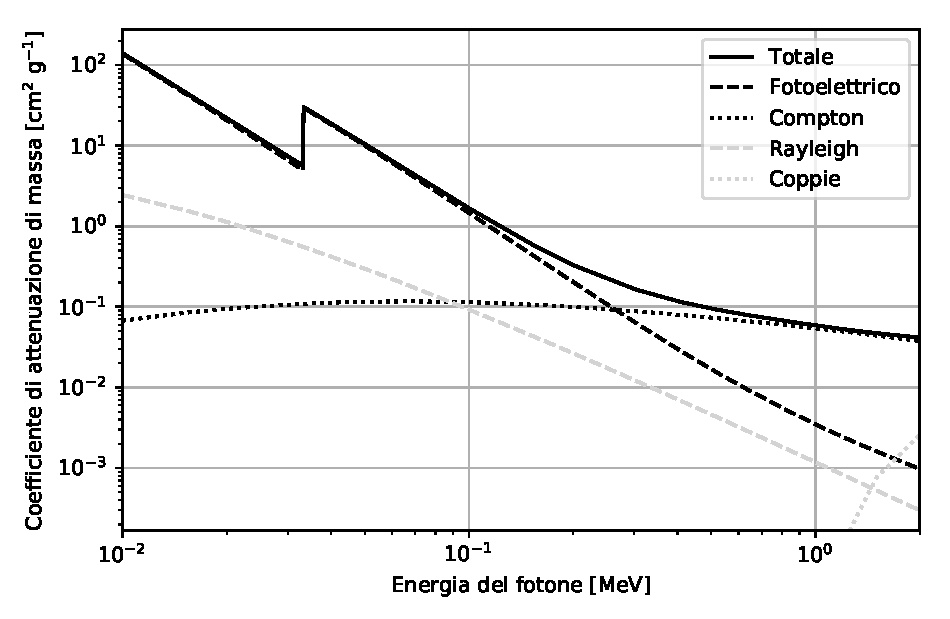
\includegraphics[width=25 em]{immagini/cross}
\caption{\label{fig:cross}
Sezioni d'urto in funzione dell'energia all'interno del nostro cristallo di NaI ($\rho=\SI{3.67}{g\,cm^{-3}})$ espressa come $\sigma=\frac{1}{\rho\lambda}$, dove $\lambda$ è il cammino libero medio all'interno del materiale. Queste informazioni sono tratte da \cite{cross}.}
\label{sezioni}
\end{figure}


\section{Apparato}

\subsection{Apparato A}

% Doveva farlo Bob.

\subsubsection{Descrizione del circuito}

Il circuito del primo apparato costruito è rappresentato in \autoref{circuitone}.

\begin{figure}[h]
\centering
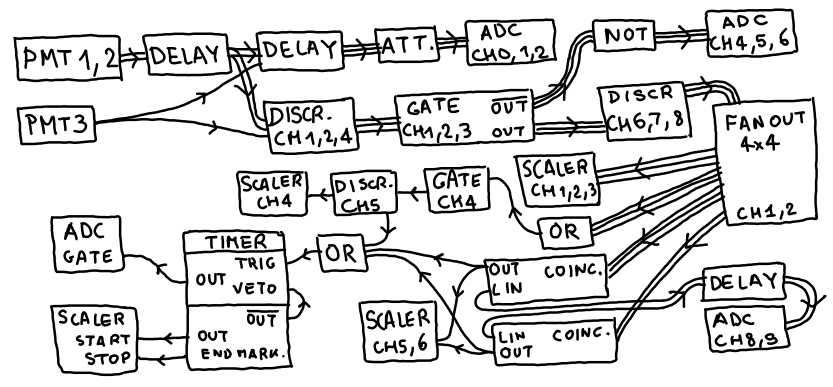
\includegraphics[width=30 em]{immagini/circuitone}
\caption{Schema circuitale dell'apparato A.}
\label{circuitone}
\end{figure}

Le uscite dei PMT sono inviate ai discriminatori, le cui uscite attraversano un modulo di antiretrigger (tempo morto di \SI{1}{\micro s}) e vengono usate per costruire funzioni logiche. I segnali dei PMT vengono anche inviati all'ADC attraverso un attenuatore per evitare di danneggiare lo strumento.
Per quanto riguarda la parte logica, costruiamo e mettiamo in tempo tre tipi di trigger:
\begin{enumerate}
\item canale
\item coincidenza a 2
\item coincidenza a 3.
\end{enumerate}
Il trigger di canale è semplicemente il segnale discriminato del PMT corrispondente; quello di coincidenze è dato dall'uscita di lunga durata del modulo stesso. Mandiamo questi segnali all'ADC in modo che il trigger di canale arrivi in contemporanea con il segnale analogico del canale stesso. Se in quel momento c'è anche un trigger di coincidenza, sappiamo se l'evento ci è arrivato da una coincidenza anziché da un canale singolo. Abbiamo fatto tutto questo per acquisire tutti i canali contemporaneamente ed agevolare la lettura dei dati via software. Purtroppo il \emph{cross-talk}%
\footnote{Spiegheremo come ci siamo accorti di questo problema nella \autoref{ref}.} presente nell'ADC ha rovinato le misure fatte con questo apparato.
Per dare precedenza agli eventi più rari abbiamo collegato questi trigger ad un modulo \emph{or} ritardando i trigger singoli rispetto a quelli di coincidenze a 2 e questi ultimi rispetto alle coincidenze a 3. L'uscita dell'\emph{or} era poi inviata ad un \emph{timer} che generava il gate dell'ADC. L'altro canale di questo \emph{timer} veniva usato per avviare o fermare le acquisizioni.

\subsubsection{Problemi riscontrati}

I problemi descritti in seguito ci hanno spinti a semplificare il circuito per cercare di risolverli.

Il più evidente fin da subito è stato il \emph{bit stuck}: il terzo bit dei dati in formato binario è sempre 1. Gli istogrammi presentano delle lacune di \SI{4}{digit} ogni \SI{4}{digit}. Risolviamo questo problema istogrammando con canali più larghi di \SI{8}{digit}.

Poi abbiamo escluso l'\emph{or} dal circuito perché i segnali che ci arrivavano dalle coincidenze mostravano avere un'energia minore. Abbiamo risolto il problema togliendo l'\emph{or} dal circuito.

Il problema più interessante è dato dal fatto che, confrontando gli spettri del \na{}, abbiamo visto che i fotoni emessi dalla sorgente con attività maggiore avevano energia maggiore.
Il grafico in \autoref{distanze} mostra l'energia dei fotopicchi del sodio in funzione della distanza della sorgente ad attività elevata dal rivelatore usato per fare la misura.
\marginpar{Sto supponendo che prima di questo punto abbiamo scritto che ci sono due sorgenti di sodio.}

\subsection{Circuito B}

Dopo aver eseguito in maniera preliminare le misure richieste, abbiamo deciso di semplificare il circuito per tenere sotto controllo le criticità descritte nella sezione precedente.

\subsubsection{Descrizione del circuito}

Il nuovo circuito segue lo schema in \autoref{circuitone}.
I segnali dei PMT vengono inviati ai discriminatori per ottenere i segnali logici e agli attenuatori per essere poi inviati all'ADC. I segnali logici attraversano un modulo di antiretrigger per poi essere usati come trigger di acquisizioni singole o per effettuare coincidenze. Una copia dei segnali finisce al contatore. Abbiamo usato il timer per far partire/fermare le acquisizioni come abbiamo fatto per il circuito precedente.

\subsubsection{Problemi riscontrati}
\label{ref}
Dopo aver acceso l'apparato il bit stuck è scomparso e l'aumento di risoluzione ci ha permesso di notare un problema che era già presente nel circuito precedente. Abbiamo iniziato a vedere uno sdoppiamento dello spettro, come evidenziato dalla \autoref{doppio}. 

\begin{figure}[h]
\centering
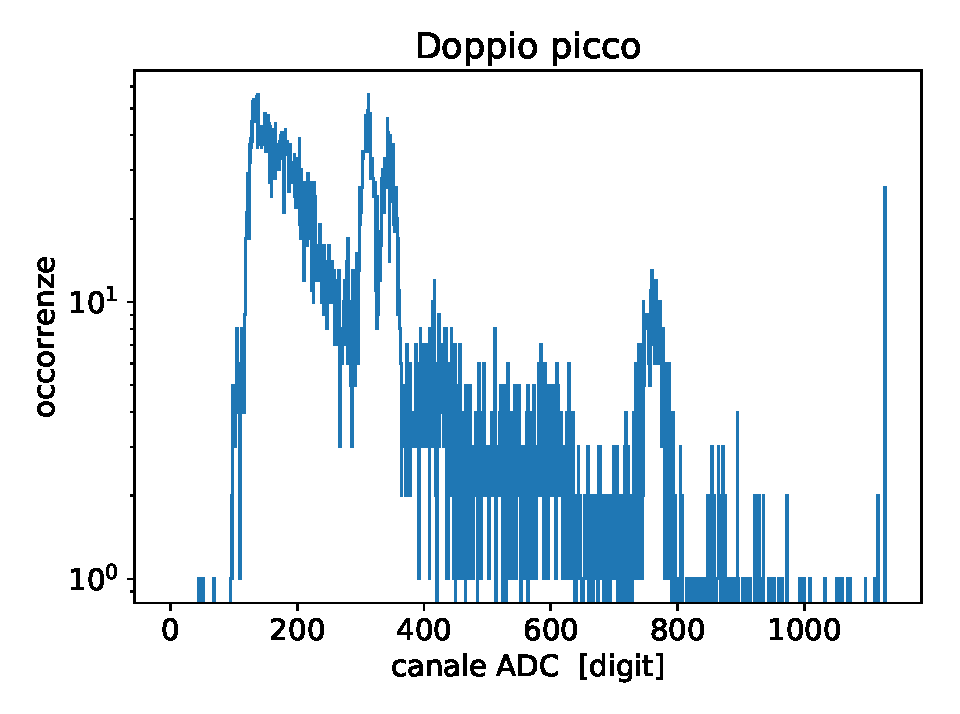
\includegraphics[width=20 em]{immagini/doppio}
\caption{Acquisizione in cui l'annichilazione presenta due picchi.}
\label{doppio}
\end{figure}

Tale problema non era visibile ad occhio nudo nelle precedenti acquisizioni, ma un fit eseguito in seguito ha mostrato la presenza di due gaussiane sovrapposte.

\marginpar{Mi pare che sia coincidenza/anticoincidenza (come detto subito dopo) che ci convince del doppio picco, non uno dei fit.
\texttt{Io mi riferivo a quella misura di stabilità in cui non si vedeva che i picchi erano 2}}

Abbiamo poi scoperto la causa del problema, ovvero il crosstalk.
Come mostra il grafico di \autoref{sdoppio} sinistra, il doppio picco è la somma di quello osservato nelle acquisizioni in coincidenza con quello osservato in anticoincidenza. 

\begin{figure}[h]
\centering
\subfloat
{
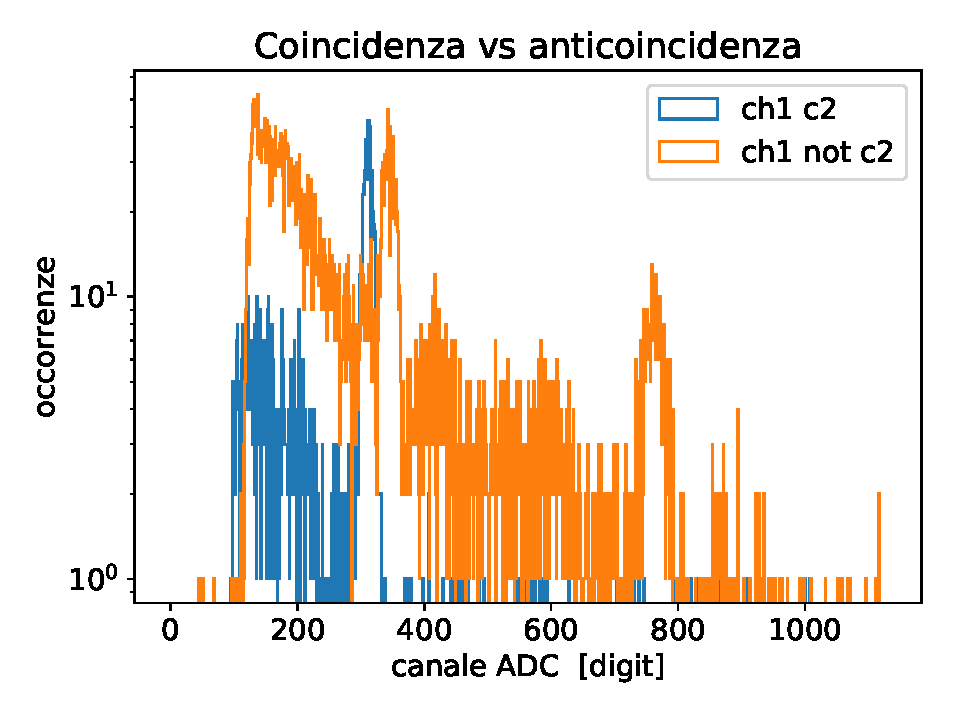
\includegraphics[width=18 em]{immagini/sdoppio}
}
\subfloat
{
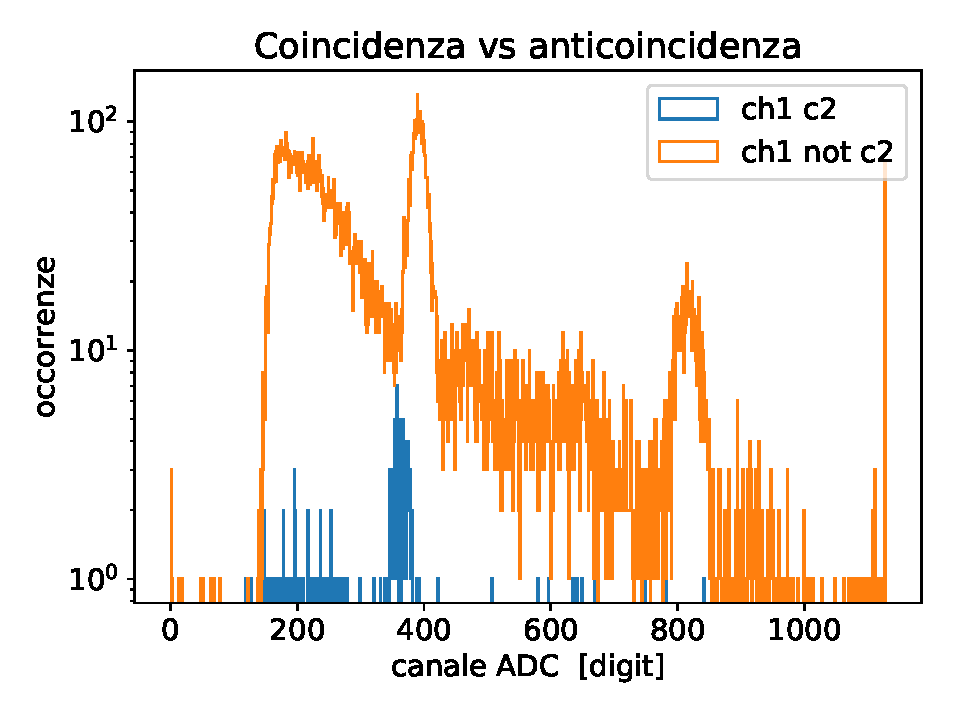
\includegraphics[width=18 em]{immagini/dist}
}
\caption{A sinistra: rappresentazione di dell'acquisizione di \autoref{doppio} separando le coincidenze dalle anticoincidenze. \\
A destra: grafico della stessa misura in cui il PMT1 è vicino alla sorgente mentre il PMT2 è lontano dalla sorgente.}
\label{sdoppio}
\end{figure}

Siamo arrivati alla conclusione che si tratti di un crosstalk dal fatto che il picco in anticoincidenza coincide con quello di un singolo canale quando tutti gli altri sono scollegati.
Inoltre abbiamo visto, aumentando la distanza di un PMT dalla sorgente, che il picco delle coincidenze si rimpicciolisce (perché ha meno eventi) e il picco in anticoincidenza tende ad assomigliare sempre di più a quello dell'acquisizione con canale singolo (\autoref{sdoppio} destra).

\marginpar{Una volta che hai separato lo spettro in coincidenza e anticoincidenza,
mi sembra inutile far vedere che le coincidenze calano se allontani i rivelatori;
sarebbe stato utile se non avessi potuto separare lo spettro.
Metterei insieme il grafico di figura 4 e il primo di figura 5 che sono il confronto interessante.}

In seguito abbiamo provato che questo problema si riscontra anche quando i canali da analizzare non sono collegati ad ingressi adiacenti dell'ADC. Inspiegabilmente, il problema si è ripresentato solo a giorni alterni. 


\section{Misura e analisi}

% Misure preliminari

\subsection{Punto di lavoro}

% Sappiamo dalla precedente esperienza sull'effetto Compton che i PMT con scintillatore di NaI(Tl) lavorano bene in un range di tensioni che va da \SI{600}V a \SI{800}V e l'unica differenza tra una tensione e l'altra è una variazione della scala.
% la frase non ha senso perché la tensione c'entra con il PMT e non con lo scintillatore.
Per i PMT scegliamo delle tensioni che seguano le caratteristiche dichiarate dal tecnico di laboratorio facendo in modo che, in presenza della sorgente, si abbiano dei rate simili tra i 3 PMT.
Allora mettiamo il PMT1 a \SI{703}V, il PMT2 a \SI{839}V ed il PMT3 a \SI{930}V.

Impostiamo le soglie dei discriminatori al minimo (circa \SI{-50}{mV}) perché il rumore casuale è
% da dove esce fuori 1 %??
%al massimo l'\SI{1}{\%} degli eventi che misuriamo usando le sorgenti meno attive
trascurabile.
% gac
%L'utilizzo delle coincidenze rende questo rumore molto più raro.

% l'abbiamo già detto nel circuito
%Usiamo degli attenuatori per cambiare la scala delle misure in caso di necessità.


\subsection{Gate dell'ADC}

Variamo la durata del gate dell'ADC e calcoliamo il rapporto $\sigma\!/$\!media per il picco di annichilazione rivelato dal PMT1, modellato come al solito con una gaussiana.
Su alcune misure abbiamo introdotto dei ritardi per migliorare o peggiorare la sincronizzazione con il gate al fine di quantificare quanto la messa in tempo influisca sulla nostra risoluzione. Il risultato di questa misura è in \autoref{fig:gate}, i dati sono in \autoref{tab:gate}.

\begin{figure}[h]
\centering
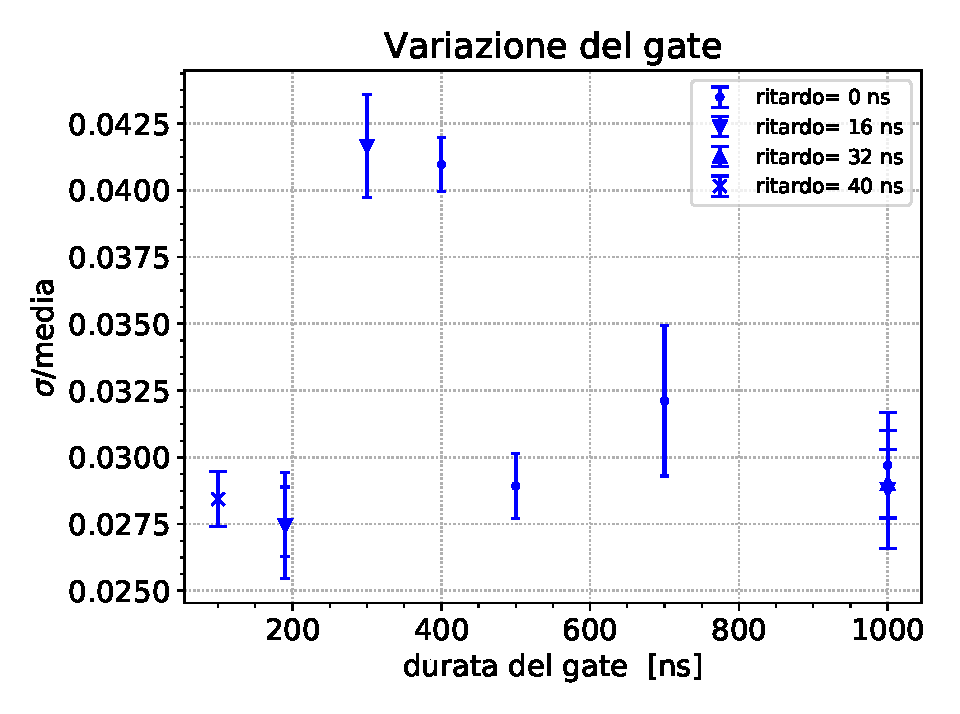
\includegraphics[width=20 em]{immagini/gate}
\caption{Grafico della risoluzione in funzione della durata del gate. Le misure sovrapposte sono state ottenute ritardando il segnale del PMT1.}
\label{fig:gate}
\end{figure}

\begin{table}[h]
\centering
\begin{tabular}{c|c|c|c}
durata (ritardo) [ns] & media [digit] & $\sigma$ [digit] & $\sigma\!/$\!media\\
\hline
 100 & 304.88$\,\pm\,$34 &  8.67$\,\pm\,$31 & 0.0284 $\,\pm\,$10 \\  
 190 & 492.82$\,\pm\,$50 & 13.59$\,\pm\,$65 & 0.0276 $\,\pm\,$13 \\
 190 & 513.05$\,\pm\,$80 & 14.1 $\,\pm\,$1.0 & 0.0274$\,\pm\,$20 \\
 300 & 307.68$\,\pm\,$36 & 12.81$\,\pm\,$59 & 0.0416 $\,\pm\,$19 \\
 400 & 344.25$\,\pm\,$25 & 14.10$\,\pm\,$34 & 0.0410 $\,\pm\,$10 \\
 500 & 524.01$\,\pm\,$42 & 15.16$\,\pm\,$64 & 0.0289 $\,\pm\,$12 \\
 700 & 482.54$\,\pm\,$85 & 15.5 $\,\pm\,$1.4 & 0.0321$\,\pm\,$28 \\
1000 & 539.43$\,\pm\,$61 & 16.0 $\,\pm\,$1.1 & 0.0297$\,\pm\,$20 \\
1000 & 553.88$\,\pm\,$71 & 15.9 $\,\pm\,$1.2 & 0.0288$\,\pm\,$22 \\
1000 & 542.68$\,\pm\,$41 & 15.75$\,\pm\,$69 & 0.0290 $\,\pm\,$13 
\end{tabular}

\caption{Andamento della risoluzione in funzione della durata del gate. I numeri tra parentesi indicano di quanto è stato ritardato il PMT1.}
\label{tab:gate}
\end{table}

Dall'analisi dei dati abbiamo potuto vedere che la risoluzione migliore si raggiunge quando il gate dura meno di \SI{200}{ns}
\marginpar{Con le incertezze riportate, mi sembra che, fatta eccezione per 300 e 400, le misure siano tutte compatibili.}
ma questo valore non è un buon punto di lavoro perché cambiare la durata del gate cambia la scala e, in questo caso, non ci permetteva di vedere il picco del neon.
\marginpar{Il motivo non è il picco del neon, perché accorciare il gate è come attenuare e quindi a maggior ragione si vedono i picchi più a destra. Inoltre usando gli attenuatori si può sempre compensare la variazione del gate.}
L'alternativa migliore sembrerebbe essere una durata del gate di \SI{1}{\micro s}, ma il manuale dell'ADC specifica che a tale valore (o anche maggiore) diminuisce la linearità della digitalizzazione. Per questo abbiamo scelto di usare un gate di \SI{550}{ns} nell'apparato A.
\marginpar{Il manuale dice che aumenta l'errore, non che peggiora la linearità (quella era per segnali sopra \SI1V). Inoltre come limite dà \SI{200}{ns}.}
Questa scelta è poi diventata \SI{1}{\micro s} nell'apparato B per evitare problemi derivanti dal jitter dei segnali. Infine notiamo che cambiare i ritardi sui segnali in ingresso non influisce significativamente sulla risoluzione dell'apparato.
\marginpar{I dati nella tabella non mi tornano. Le sigma sono grosse quanto le medie e infatti i rapporti vengono tutti dell'ordine dell'unità, diversi da quelli riportati nel grafico.}


\subsection{Stabilità}

Mostriamo l'instabilità del nostro sistema di rivelatori nei 2 apparati sopra descritti monitorando la posizione dei fotopicchi del sodio in funzione del tempo.
La prima misura è stata fatta con l'apparato A il 3 maggio e dura \SI{16}{ore}, la seconda  è stata eseguita con l'apparato B il 15 maggio e dura \SI{63}{ore}.
Nella prima misura sono presenti tutti i canali, nella seconda è presente solo il canale 1 per evitare il cross-talk riscontrato nella precedente.
Abbiamo usato l'energia nominale dei 2 picchi per ricavare una ``retta di calibrazione'' di pendenza $m$ e intercetta $q$ e abbiamo osservato l'evoluzione temporale di questi parametri. Usiamo l'espressione tra virgolette perché lo scopo dell'esperienza è fingere di non conoscere la massa dell'elettrone per poi misurarla.

% misura 1
\begin{figure}[h]
\centering
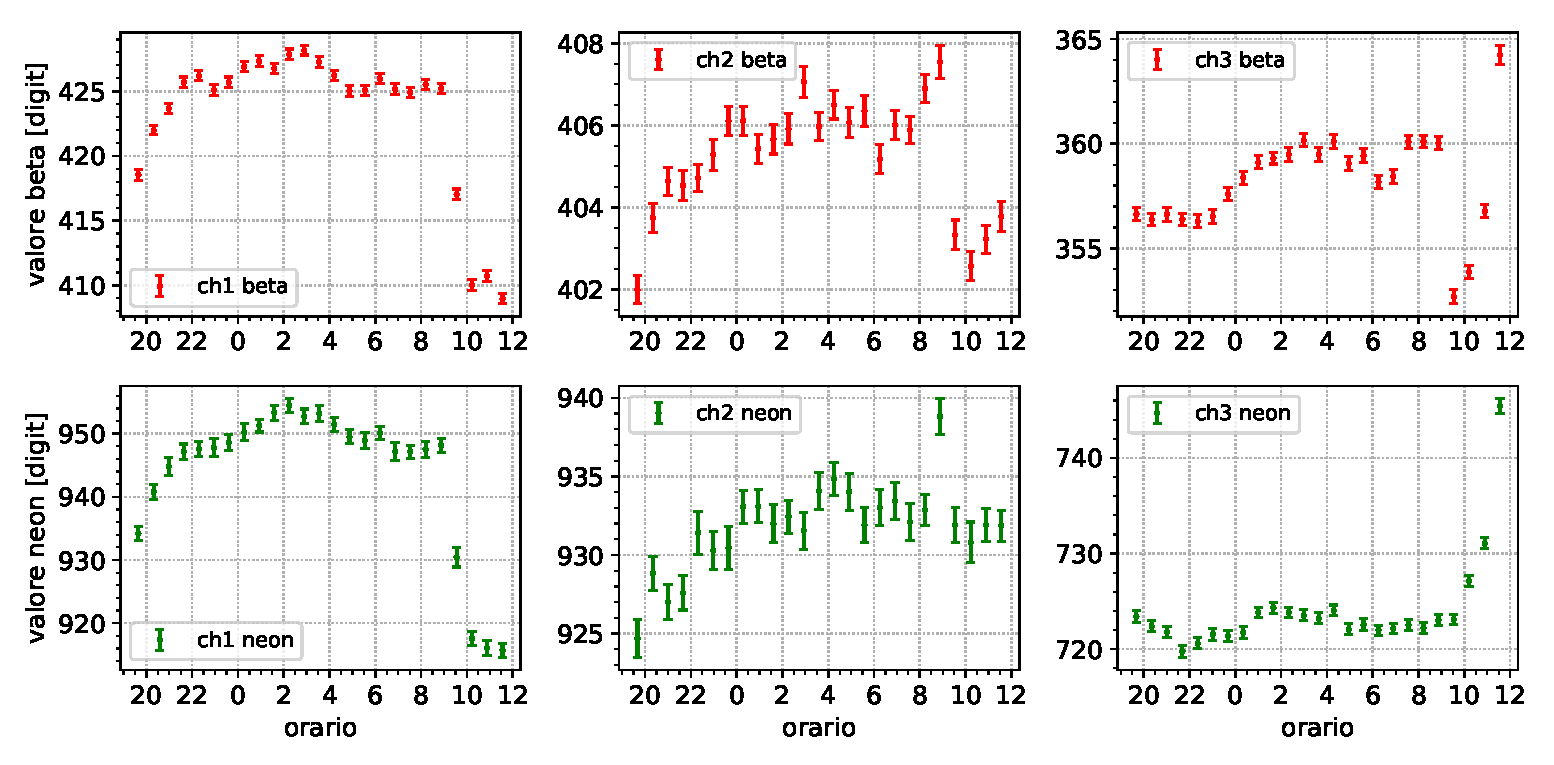
\includegraphics[width=\textwidth]{immagini/0503_picchi}
\caption{Misura di stabilità iniziata il 3 maggio alle 19. I grafici rappresentano la posizione dei picchi in funzione del tempo; ``beta'' indica il picco di annichilazione e ``neon'' indica il fotone emesso dal decadimento del neon.}
\label{picchi1}
\end{figure}

\begin{figure}[h]
\centering
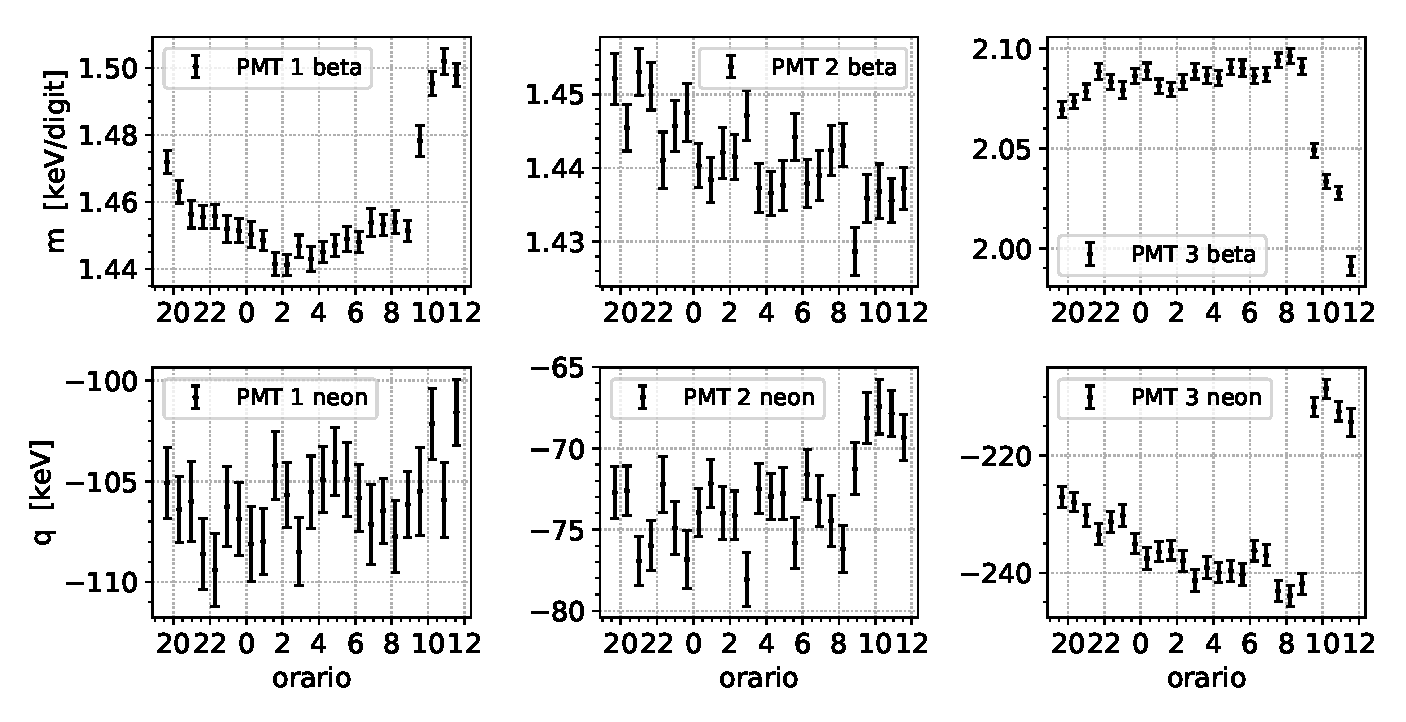
\includegraphics[width=\textwidth]{immagini/0503_rette}
\caption{Misura di stabilità iniziata il 3 maggio alle 19. I grafici rappresentano il valore della pendenza e dell'intercetta della ``retta di calibrazione'' in funzione del tempo.}
\label{rette1}
\end{figure}

% misura 2
\begin{figure}[h]
\centering
\subfloat
{
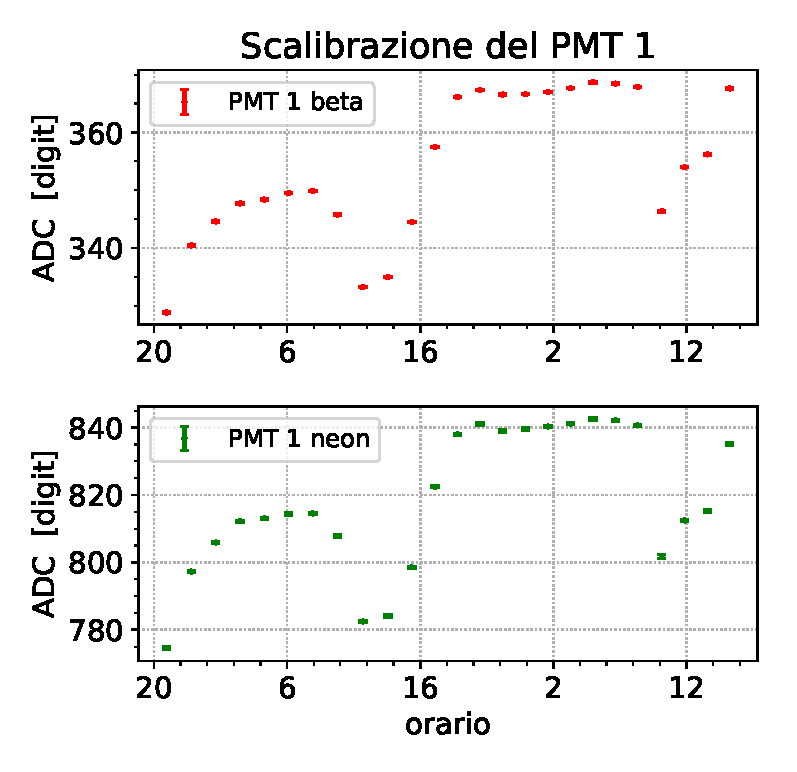
\includegraphics[width=0.49\textwidth]{immagini/0515_picchi}
}
\subfloat
{
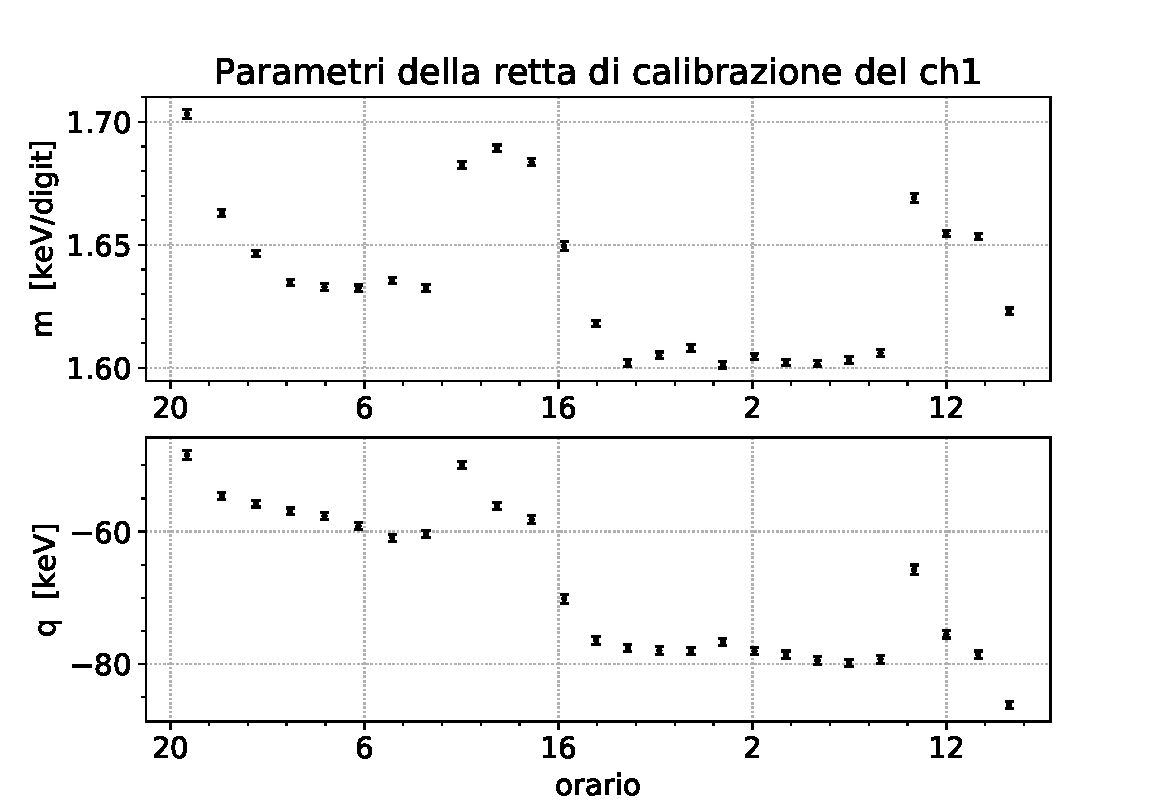
\includegraphics[width=0.49\textwidth]{immagini/0515_rette}
}
\caption{Misura di stabilità iniziata il 15 maggio alle 19.\\
A sinistra:  grafici che rappresentano la posizione dei picchi in funzione del tempo; ``beta'' indica il picco di annichilazione e ``neon'' indica il fotone emesso dal decadimento del neon. \\
A destra: grafici che rappresentano il valore della pendenza e dell'intercetta della ``retta di calibrazione'' in funzione del tempo.}
\label{picchi2}
\end{figure}

% discussione dei dati
Guardando i dati della prima misura (\autoref{picchi1} e \autoref{rette1}) vediamo che i vari rivelatori si scalibrano in modo diverso. L'andamento dei punti indica la notte come momento di massima stabilità e l'apertura del laboratorio come momento di massima instabilità.

Dai dati della seconda misura (\autoref{picchi2} sinistra e \autoref{picchi2} destra) si nota uno spostamento coerente dei fotopicchi del sodio che si stabilizza durante la notte. Anche qui si nota una scalibrazione significativa durante gli orari di apertura del laboratorio.
Le stesse considerazioni valgono anche per i parametri della retta di calibrazione.

\subsection{Rimbalzi}

Guardando lo scatter plot di misure in coincidenza, abbiamo notato dei comportamenti non attesi che abbiamo supposto e poi verificato essere dei fotoni che rimbalzano da un rivelatore all'altro.

La \autoref{scatter} mostra un tipico scatter plot nella configurazione in cui 2 rivelatori sono posti uno di fronte all'altro alla stessa distanza da una sorgente di \na{}.

\begin{figure}[h]
\centering
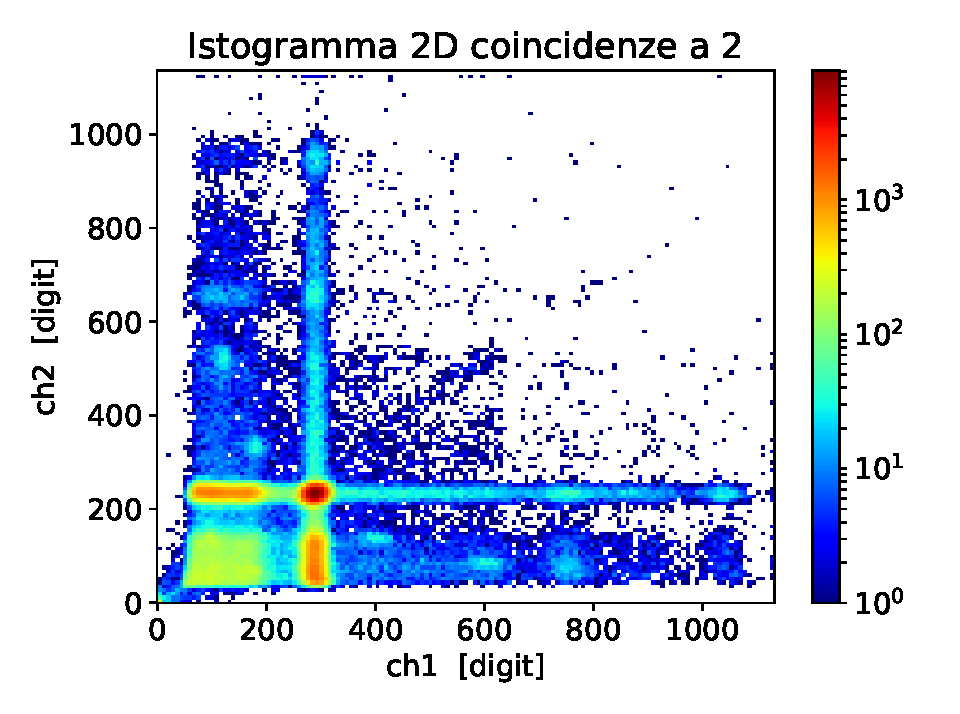
\includegraphics[width=\textwidth]{immagini/esempio}
\caption{Tipico scatter plot di una misura in coincidenza. La descrizione di questo grafico è presente nel testo.}
\label{scatter}
\end{figure}

\marginpar{Chiedere a Jack di fare il super grafico con istogrammi 1D e 2D se non si perde troppo tempo}

Si vedono degli eccessi in alcuni punti del grafico che chiameremo in seguito \emph{strutture}. La più vistosa si manifesta quando entrambi i fotoni di annichilazione effettuano un processo fotoelettrico all'interno degli scintillatori. In basso a sinistra si nota invece la zona in cui entrambi hanno subito una diffusione Compton. Le bande arancioni intorno a questa zona rappresentano invece gli eventi in cui un fotone proveniente dall'annichilazione ha fatto fotoelettrico su un rivelatore e l'altro ha fatto Compton sull'altro.
La stessa cosa avviene con il fotone proveniente dal decadimento del neon, rappresentato dalle strutture nella parte centrale del grafico adiacente ai bordi della figura. La struttura più a destra (o più in alto) rappresenta l'arrivo simultaneo di un fotone di annichilazione insieme ad uno del neon. L'interpretazione degli eventi è analoga a quelli descritti precedentemente.

\marginpar{Non sarebbe male mettere una legenda sui picchi.}

Le strutture non attese sono i due eccessi presenti nella zona in cui il fotone del neon e quello dell'annichilazione fanno entrambi scattering Compton. Queste strutture si manifestano a valori di energia coincidenti ai picchetti della spalla Compton
\marginpar{``Picchetti della spalla Compton'' non è molto chiaro, ma ci penserò più tardi a come aggiustarli.}

Per verificare la nostra ipotesi abbiamo messo i rivelatori nella configurazione di \autoref{spostati}, in modo da poterci aggiungere dei mattoni di piombo come in \autoref{spostati2}. \marginpar{AGGIUSTARE}
Lo scatter plot corrispondente si trova in \autoref{spostato}: la struttura più popolata non è più data dalla rivelazione simultanea dell'annichilazione per effetto fotoelettrico, ma dalla somma degli eventi nelle bande che si incrociano.
In questa configurazione non si nota più uno degli eccessi inattesi nominati prima: quello ad energia più alta. Adesso sono diventate evidenti due strutture circolari nella zona in basso a sinistra del grafico: esse e l'ultimo tipo di struttura rimasta scompaiono completamente quando effettuiamo la misura nella configurazione mostrata in \autoref{spostati2}, come mostrato in \autoref{piombo}.

\begin{figure}[h]
\centering
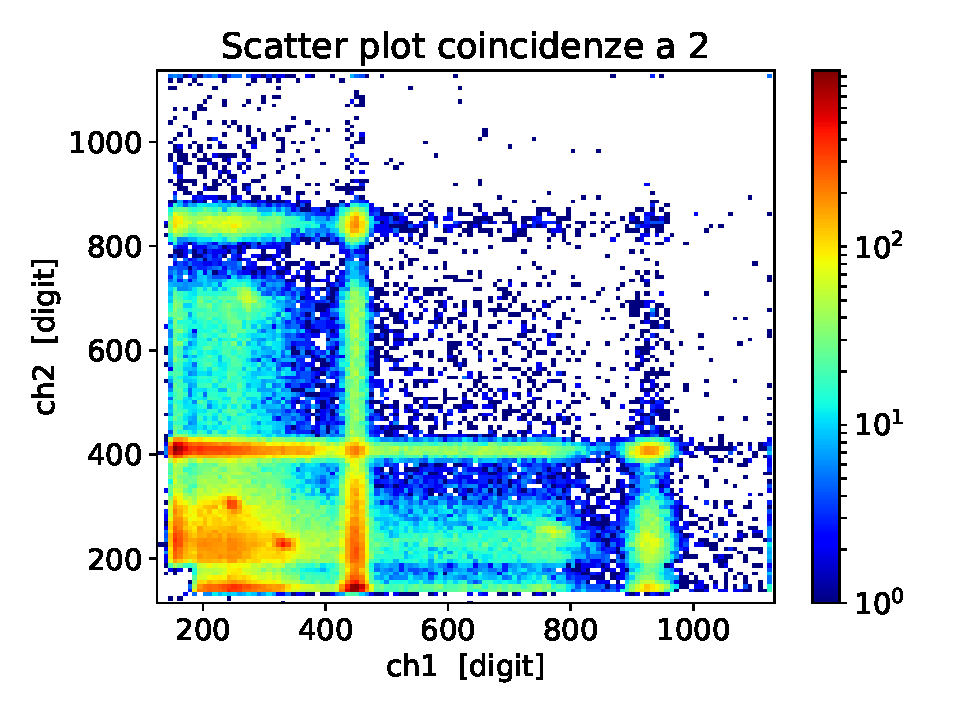
\includegraphics[width=\textwidth]{immagini/0518_rimbalzi}
\caption{Misura eseguita nella configurazione di \autoref{spostati}. La descrizione del grafico è presente nel testo.}
\label{spostato}
\end{figure}

\begin{figure}[h]
\centering
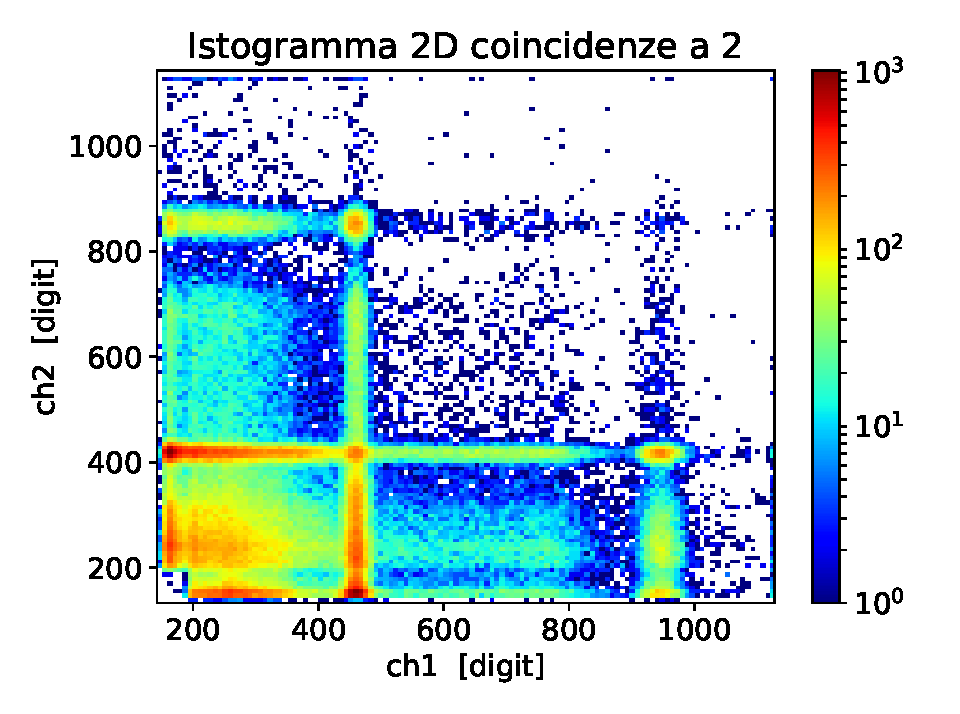
\includegraphics[width=\textwidth]{immagini/0518_piombo}
\caption{Misura eseguita nella configurazione di \autoref{spostati2}. La descrizione di questo grafico è presente nel testo.}
\label{piombo}
\end{figure}


\subsubsection{Misura con un solo fotone}

Abbiamo effettuato la misura nella configurazione di \autoref{solo} e poi \autoref{solo_pb} usando la sorgente di \cs{}: lo scopo della misura è quantificare l'importanza di un rimbalzo tra scintillatori vicini.

 


\subsection{Misure con TDC}

Collegando le uscite discriminate dei PMT 1 e 2 ai due ingressi dell'unico TDC funzionante che abbiamo trovato in laboratorio, possiamo misurare i ritardi tra le risposte di due PMT posti uno di fronte all'altro sfruttando i fotoni dell'annichilazione. Per eseguire la misura usiamo come trigger le coincidenze e ritardiamo i segnali dei due PMT, dato che il trigger è successivo alla rivelazione dei fotoni. \`E stato scelto un ritardo di \SI{60}{ns} in modo che la differenza tra i tempi di arrivo $\Delta t=t_1-t_2$ possa essere sia positiva che negativa.

Prima di eseguire la misura calibriamo il TDC con il generatore di funzioni usando come trigger un'onda quadra e come \emph{stop} lo stesso segnale ma ritardato in modo arbitrario.
Eseguiamo questa calibrazione per le due scale disponibili: \SI{102}{ns} e \SI{510}{ns}.
Le calibrazioni hanno mostrato una buona linearità, ma la misura dei ritardi ha mostrato che il TDC, per un motivo a noi ignoto, non funziona.
Il grafico di Figura\autoref{100} è uguale a quello di Figura\autoref{500} nonostante le acquisizioni siano state fatte con due scale diverse. Se nei due grafici ci fosse la stessa cosa, vedremmo la figura allargata di un fattore dato dal rapporto dei due fondoscala. Inoltre l'offset delle scale del TDC vale circa \SI{1}{digit}, quindi lo spostamento di circa \SI{50}{digit} del picco presente nei grafici non può essere spiegato da nessun effetto fisico.

\begin{figure}[h]
\centering
\subfloat
{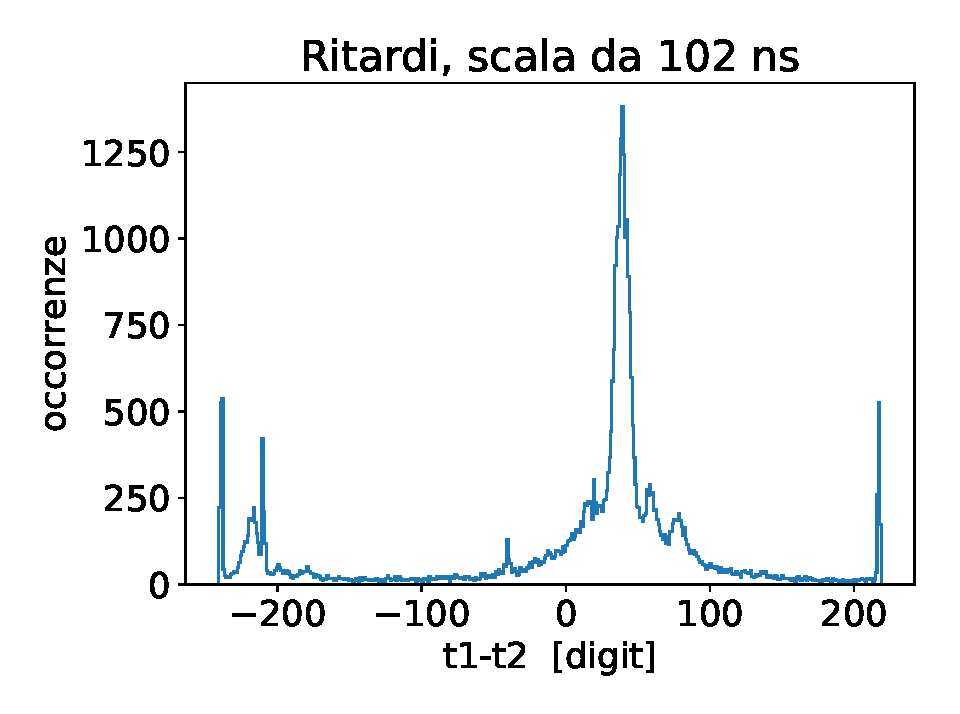
\includegraphics[width=17 em]{immagini/100}
\label{100}} \quad
\subfloat
{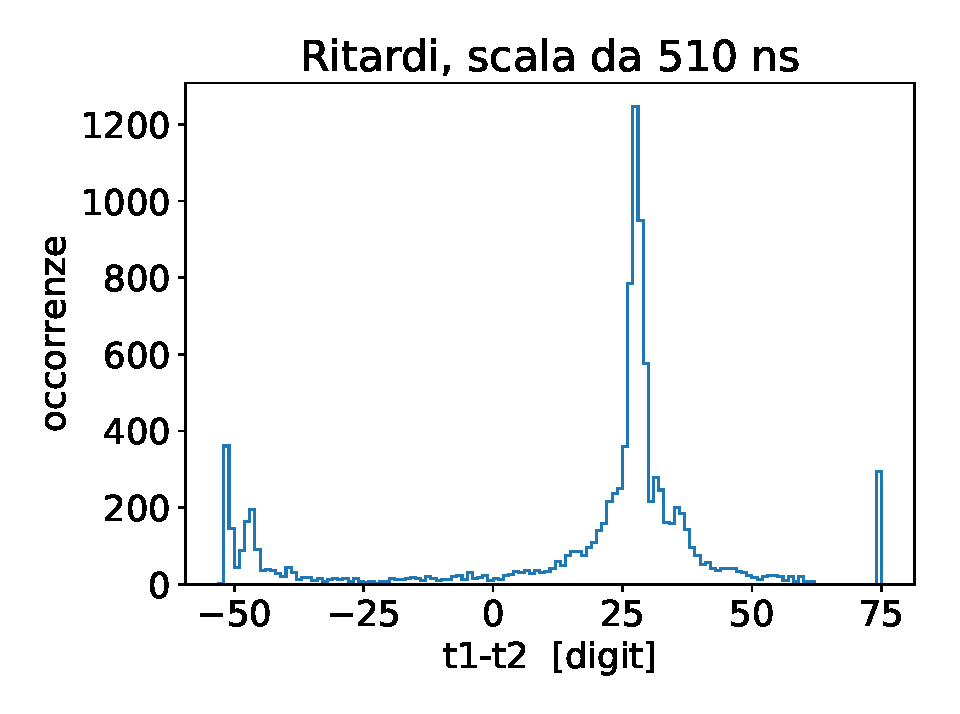
\includegraphics[width=17 em]{immagini/500}
\label{500}}

\caption{Misura di ritardo vista da entrambe le scale del TDC.}
\label{confronto}
\end{figure}

Questo problema ci impedisce di fare i facoltativi.

% Misure importanti

\subsection{Massa dell'elettrone}

Per ricavare la massa dell'elettrone misuriamo l'energia del picco di annichilazione del \na{}
calibrando la scala di energia con i fotopicchi di \co{} e \cs{}.
Poiché la scala di energia varia significativamente nell'arco di tempo in cui facciamo le misure,
misuriamo contemporaneamente lo spettro di tutte le sorgenti.
Triggeriamo su un singolo PMT,
collegando solo quel PMT all'ADC, per evitare il crosstalk tra i canali dell'ADC.
Ripetiamo la misura con i 3 scintillatori disponibili.

\subsubsection{Fit dei picchi}

\begin{figure}
	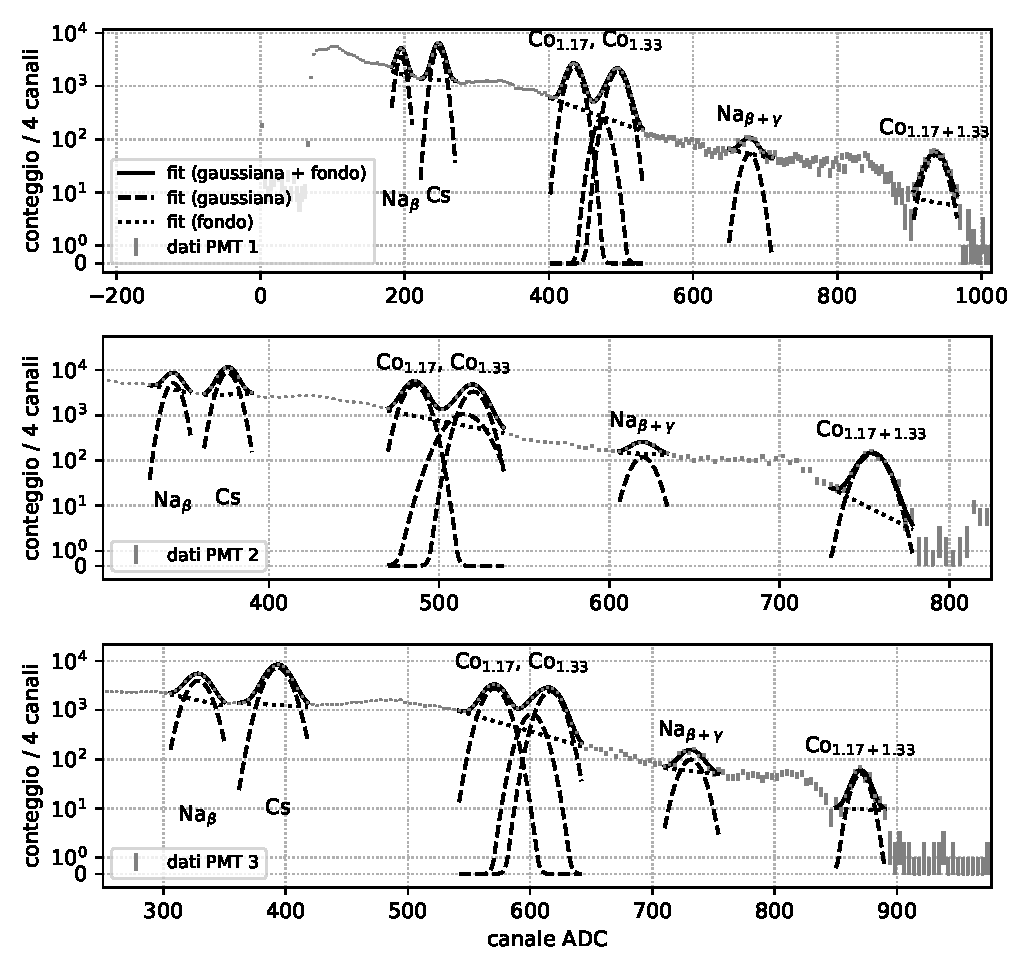
\includegraphics[width=\textwidth]{immagini/mass18-peaks}
	\caption{\label{fig:mass18-peaks}
	Ciao}
\end{figure}

Fittiamo ogni picco, scegliendo a mano l'intervallo di canali su cui fittare,
con una gaussiana più un esponenziale come fondo.
Il fit è ai minimi quadrati sull'istogramma.
I bin fittati contengono tutti almeno 5 eventi.
Controlliamo che cambiare il ribinnaggio dei canali dell'ADC non cambia significativamente il risultato.
I~fit sono riportati in \autoref{fig:mass18-peaks}.
Tutti i fit hanno un pvalue ragionevole;
il test di Kolmogorov-Smirnov sull'uniformità dei pvalue dà un pvalue \SI{18}\%.
Per i picchi del cobalto e quello del neon, che sono sovrapposti, il fit è unico.
Con dei test vediamo che il risultato per la media del picco del neon,
che è praticamente nascosto da quelli del cobalto,
è instabile, quindi lo teniamo nel fit come fondo ma non lo usiamo per ricavare la massa.

\subsubsection{Fit della massa}

\begin{figure}
	\centering
	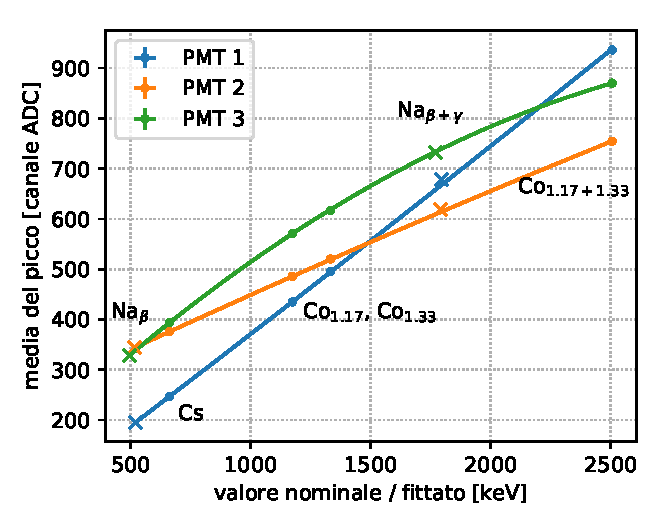
\includegraphics[width=25em]{immagini/mass18-cal}
	\caption{\label{fig:mass18-cal}
	Ciao}
\end{figure}

\begin{table}
	\hspace{-3em}
	\begin{tabular}{c|cccc|cc}
		PMT & $a$ & $b$ [\si{keV^{-1}}] & $c$ [\si{keV^{-2}}] & $m$ [\si{keV}] & $\chi^2$/dof & $F$ \\
		\hline
		1 &   \num{7.31(54)} &  \num{0.3584(11)} &   \num{2.60(26)} & \num{519.95(50)} & 33.3 & 6.9 \\
		2 & \num{228.02(31)} & \num{0.22802(56)} &  \num{-3.55(11)} & \num{516.44(55)} & 24.4 & 6.2 \\
		3 & \num{113.47(44)} & \num{0.46701(84)} & \num{-32.94(18)} & \num{495.25(44)} &  4.1 & 2.3
	\end{tabular}
	\caption{\label{tab:massfit}
	Risultati dei fit di calibrazione e massa dell'elettrone per ogni PMT.
	La curva di calibrazione è $E_\text{adc}=2cE^2+bE+a$.
	In tutti i fit le correlazioni risultano circa \SI{50}\% tra $m$ e gli altri parametri
	e circa \SI{95}\% tra $a$, $b$ e $c$.
	$F$ è il fattore per cui riscalare l'incertezza su $m$
	ricavato testando il fit sui picchi di calibrazione.}
\end{table}

Inizialmente fittiamo le medie dei picchi in funzione dell'energia con una retta
\begin{equation}
	\label{eq:retta}
	E_\text{adc} = b \cdot E + a,
\end{equation}
dove, a seconda dei casi, $E$ è
\begin{itemize}
	\item il valore noto dell'energia per i picchi di calibrazione;
	\item la massa $m$ dell'elettrone (parametro di fit) per il picco di annichilazione;
	\item $m$ più l'energia del fotone del neon per il picco $\na_{\beta+\gamma}$.
\end{itemize}
Nel fit teniamo conto della correlazione tra i picchi del cobalto.
Il pvalue del fit è praticamente 0,
ovvero le incertezze statistiche sono sufficientemente piccole da rigettare il modello \eqref{eq:retta}.

Poiché abbiamo ancora 3 gradi di libertà,
rendiamo il modello più generico aggiungendo il termine quadratico:
\begin{equation}
	\label{eq:parabola}
	E_\text{adc} = 2c \cdot E^2 + b \cdot E + a.
\end{equation}
Anche questo modello viene rigettato con forza per i PMT 1 e 2, ma non per il 3.
Non vogliamo avere meno di due gradi di libertà nel fit,
quindi in mancanza di un modello adeguato stimiamo un'incertezza sistematica aggiuntiva in questo modo:
per ogni picco di calibrazione ripetiamo il fit lasciando libera,
oltre all'energia del picco di annichilazione,
anche l'energia del picco di calibrazione.
Per ognuno di questi fit calcoliamo il rapporto tra
la differenza tra l'energia fittata e l'energia nota del picco di calibrazione
e la deviazione standard stimata dal fit sull'energia fittata.
Riscaliamo l'incertezza sulla massa del fit principale
per la media quadratica di questi rapporti.
Il grafico del fit è riportato in \autoref{fig:mass18-cal},
i risultati dettagliati sono riportati in \autoref{tab:massfit}.
Le masse fittate, con l'incertezza riscalata, risultano
\begin{center}
	\begin{tabular}{cc}
		PMT 1: & $m=\SI{520.0(34)}{keV}$ \\
		PMT 2: & $m=\SI{516.4(34)}{keV}$ \\
		PMT 3: & $m=\SI{495.2(10)}{keV}$
	\end{tabular}
\end{center}


\subsection{Annichilazione in 3 fotoni}

%teoria
\subsubsection{Stime teoriche}
Lo scattering $e^+e^-$ può produrre uno stato finale con 3 fotoni: il rapporto teorico dei branching ratio tra questo processo e la più comune annichilazione in 2 fotoni è $\sim 1/378$ \cite{4}. La distribuzione angolare attesa per i 3 fotoni prodotti è rappresentata in \autoref{fig:3gamma_angular_distr}. Se il decadimento avviene a riposo nel sistema del laboratorio i fotoni sono vincolati ad essere emessi su un piano: quindi fissata la direzione di 2 fotoni, il terzo è vincolato ad essere emesso su un arco di circonferenza i cui limiti sono fissati dalla conservazione dell'energia. A causa di questi vincoli e poiché i nostri spettrometri rivelano solo in un certo angolo solido, il rate dei conteggi per questo tipo di segnale sarà inversamente proporzionale a $d^5$ dove $d$ è la distanza dei rivelatori (nel caso semplice in cui sono alla stessa distanza).
Come visibile in \autoref{fig:3gamma_angular_distr} la probabilità relativa di emissione varia poco negli angoli permessi (variazione massima del $\sim 25\%$) e per i nostri scopi è ragionevolmente uniforme per angoli intorno a $\alpha\simeq \SI{120}{\degree}$ e $\beta\simeq\SI{120}{\degree}$.
Le energie dei 3 fotoni al variare degli angoli sono facilmente ricavabili dalla conservazione del quadrimpulso:
\begin{align*}
\label{eq:3gamma_energy}
E_3 &= \frac{2 m_e}{\frac{\sin\beta \;+\;(1+\cos\alpha)}{\sin\alpha}+\cos\beta+1}\\
E_2 &= E_3 \cdot \frac{\sin\beta}{\sin\alpha}\\
E_1 &= 2m_e - E_2 - E_3\\
\end{align*}
dove $\alpha$ e $\beta$ sono rispettivamente i supplementari degli angoli tra il fotone 1 e i fotoni 2 e 3
(convenzione differente da quella di \autoref{fig:3gamma_angular_distr}).

\begin{figure}[h]
	\centering
	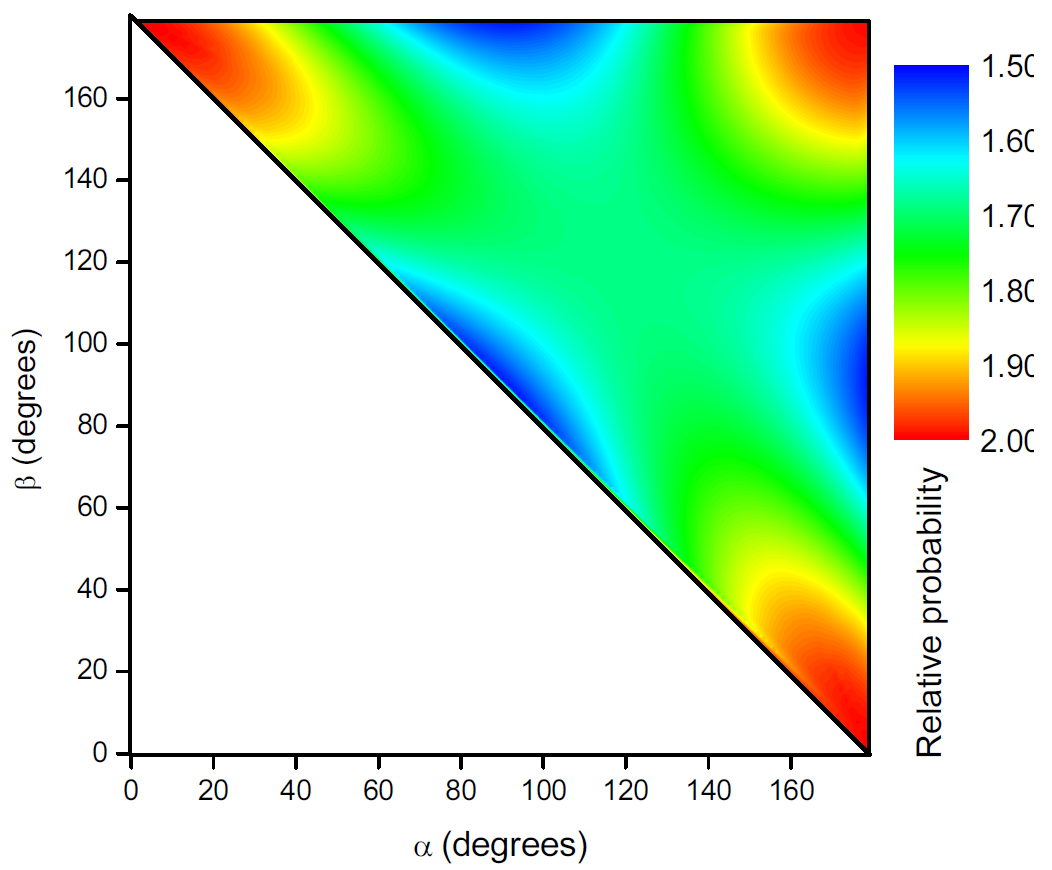
\includegraphics[width=20em]{immagini/3gamma_distribution}
	\caption{\label{fig:3gamma_angular_distr}Probabilità di una data distribuzione angolare per l'annichilazione a 3 fotoni \cite{4}. $\alpha$ e $\beta$ sono rispettivamente gli angoli tra il fotone 1 e i fotoni 2 e 3
	(sono diversi dagli $\alpha$ e $\beta$ definiti in questa relazione).
	La scala della probabilità e arbitraria.}
\end{figure}
%progettazione dell'esperimento

Una stima dell'ordine di grandezza del numero di eventi di segnale attesi è ottenibile a partire dalla formula:
\begin{equation}
\label{eq:stima_3gamma}
N_{3\gamma} \simeq T \cdot R_{\beta^+} \cdot \frac{\text{BR}(3\gamma)}{\text{BR}(2\gamma)} \cdot \text{Acc} \cdot \text{Eff} \cdot R_{p2t}
\end{equation}
Dove:
\begin{itemize}
	\item $T$ è il tempo di presa dati, realisticamente dell'ordine di $\SI{10}{h}$;
	\item $R_{\beta^+}$ è il rate di emissione di positroni della nostra sorgente principale, dell'ordine di $\SI{500}{kBq}$;
	\item $\frac{\text{BR}(3\gamma)}{\text{BR}(2\gamma)}$ è il rapporto dei branching ratio dei due processi ed è atteso essere $1/378$;
	\item Acc è l'accettanza combinata dei tre rivelatori che possiamo stimare in $\sim 3!\frac{r^5}{2^7 d^5}$ (questa è solo una stima dell'integrale dello spazio delle fasi a 3 corpi) dove $r$ è il raggio dei rivelatori ($1''$) e che ad una distanza di $\SI{20}{cm}$ dà un'accettanza del $\sim\SI{1.2e-6}{}$;
	\item Eff è l'efficienza intrinseca combinata dei tre spettrometri che per rivelatori di NaI $2''\times2''$ è nota \cite{3} e all'energia di $\sim \SI{300}{keV}$ vale circa $(90\%)^3 \simeq  70\%$;
	\item $R_{p2t}$ è il rapporto tra gli eventi nel picco fotoelettrico e il totale, anche questo noto \cite{3} e alla stessa energia vale circa $(60\%)^3 \simeq 20\%$.
\end{itemize}
\subsubsection{Rumore}
Il risultato della stima è circa 10 eventi. A questo punto è necessario stimare/misurare il rumore.
Il rate di coincidenze a 3 in alcune configurazioni provate è in ogni caso molto maggiore del segnale atteso è quindi necessario ottimizzare il rapporto segnale/rumore per rendere visibile il segnale.
Le coincidenze casuali sono depresse dal fatto che si tratta di una coincidenza a tre; la fonte principale di rumore è la sorgente stessa: 
anche se la sorgente non si trova sulla congiungente di nessuna coppia di rivelatori, rendendo di fatto impossibile rilevare direttamente la coppia di fotoni back-to-back prodotti nell'annichilazione, è comunque possibile che la coincidenza a tre scatti e possa esserci un evento indistinguibile dal segnale.
Indicando con $\gamma_{\text{Ne}}$ i fotoni prodotti dal decadimento del $^{22}\text{Ne}$ e con $\gamma_{\beta}$ quelli prodotti dall'annichilazione in due fotoni, si ha ad esempio:
\begin{enumerate}
	\item il $\gamma_{\text{Ne}}$ passa per il rilevatore 1 e ci interagisce facendo scattering Compton;
	\item un $\gamma_{\beta}$ fa scattering Compton nel rivelatore 2;
	\item l'altro $\gamma_{\beta}$ fa scattering Compton o Rayleigh nel materiale che circonda la sorgente (la scatola di metallo che la contiene, il piombo e le pareti in piombo nelle vicinanze) venendo deviata e successivamente interagisce nel rivelatore~3.
\end{enumerate}
Un evento del genere farebbe scattare la coincidenza e al variare degli angoli di scattering potrebbe portare ad un evento simile al segnale per energia rilasciata nei rivelatori. Un'altro possibile evento di rumore è quello in cui:
\begin{enumerate}
	\item un $\gamma_{\beta}$ fa scattering Compton nel rivelatore 1 e l'altro è perso;
	\item il $\gamma_{\text{Ne}}$ fa scattering Compton nel rivelatore 2 e il fotone uscente dal processo di scattering interagisce con il rivelatore~3.
\end{enumerate}
Chiaramente molti altri possibili rimbalzi sono possibili e possono risultare simili al segnale, ma ogni rimbalzo riduce sostanzialmente la probabilità dell'evento: un ``rimbalzo'' dal rivelatore 2 al 3 come nell'esempio precedente è soppresso dal fatto che il back-scattering Compton è sfavorito e dall'accettanza del rivelatore 3 visto dal 2 che, in prima approssimazione, va come $\frac{1}{(2d)^2}$.
Un metodo per misurare il rumore dovuto alla sorgente, eliminando solo il segnale dell'annichilazione in $3\gamma$, è quello di sollevare/abbassare la sorgente in modo tale che nessun piano possa passare per la sorgente e i tre rivelatori: questo eliminerà il segnale fisico lasciando ragionevolmente immutata la forma del rumore.
\subsubsection{Realizzazione della misura}
Si sono adottati alcuni accorgimenti per migliorare il rapporto segnale rumore:
\begin{itemize}
	\item per aumentare il segnale mettiamo gli scintillatori il più vicino possibile alla sorgente: il segnale cresce con l'inverso di $d^5$ quindi passando da $\SI{20}{cm}$ a $\SI{10}{cm}$ si guadagna un fattore 32;
	\item aspettandoci che i rimbalzi tra un rivelatore e l'altro possano rappresentare una parte rilevante del rumore interponiamo dei blocchi di piombo tra un rivelatore e l'altro, abbastanza spessi da fermare la maggior parte dei fotoni (la lunghezza di interazione per energie nel range $\SI{300/500}{keV}$ è $\sim \SI{0.5}{cm}$ e si sono usati blocchi da $\sim \SI{4}{cm}$);
	\item dopo aver osservato la distribuzione tipica del rumore decidiamo gli angoli a cui effettuare la misura di segnale in modo che l'energia dello stesso sia nella zona con meno rumore possibile.
\end{itemize}

La misura finale è stata presa nelle condizioni schematizzate in \autoref{fig:schema3gamma} e riproposta nella foto in \autoref{fig:foto_3gamma}, dove sono chiari i vincoli imposti dall'apparato: i PMT 1, 2 e 3 distano rispettivamente $\SI{10.4(1)}{cm}$, $\SI{9.4(1)}{cm}$ e $\SI{11.0(1)}{cm}$  dalla sorgente e $\alpha \simeq \SI{59(1)}{\degree}$ e $\beta \simeq \SI{43(1)}{\degree}$. Il picco delle energie attese dei tre fotoni sono $E_1= \SI{397}{keV}$, $E_2 =\SI{277}{keV}$, $E_3=\SI{347}{keV}$.
 \begin{figure}[h]
	\centering
	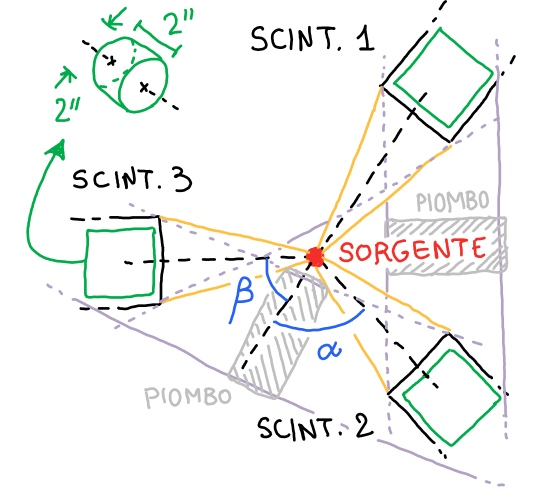
\includegraphics[width=20em]{immagini/schema3gamma}
	\caption{\label{fig:3gamma_signal} Schema dell'apparato utilizzato per la misura del rate di annichilazione in tre fotoni.}
	\label{fig:schema3gamma}
\end{figure}
Sono state realizzate due prese dati di segnale e una di rumore: sono state svolte quando il laboratorio è chiuso e la risposta dei rivelatori è stabile, con lo stesso obiettivo la parte iniziale e finale della presa dati è stata tagliata: il risultato sono due misure di segnale da $\SI{9.7}{h}$ e $\SI{15.3}{h}$ e una di rumore da $\SI{11.1}{h}$.
 \begin{figure}[h]
	\centering
	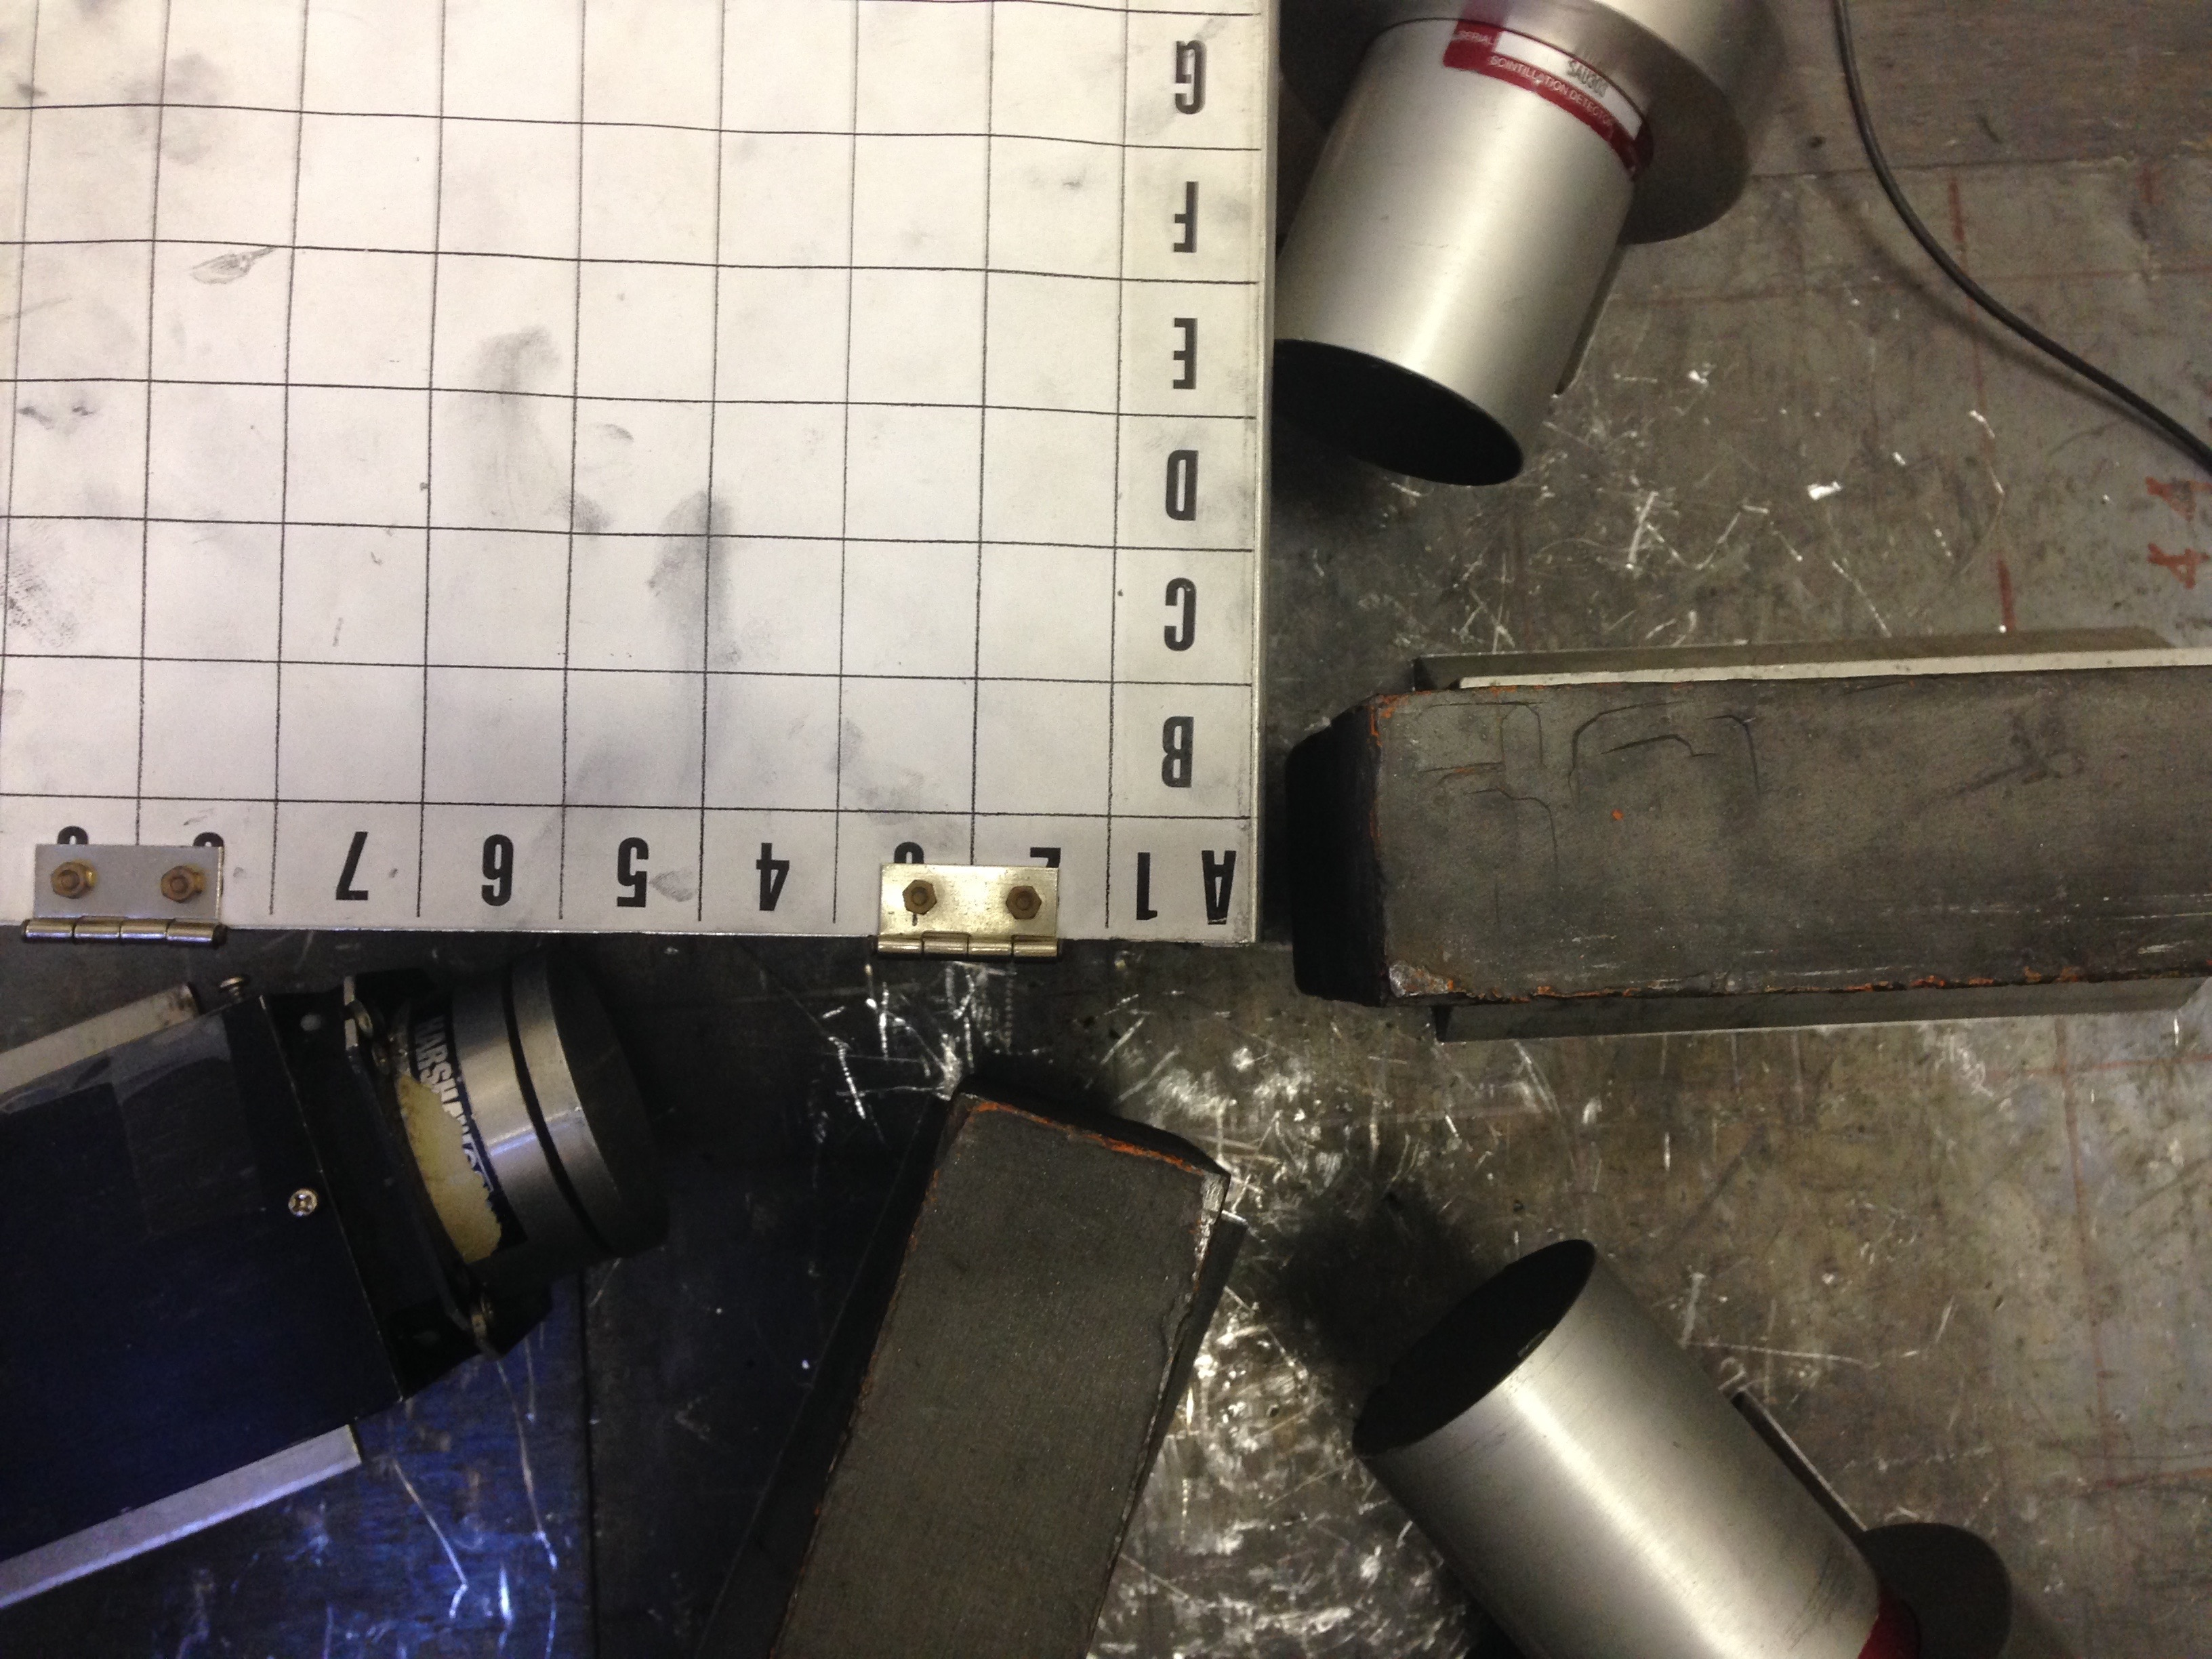
\includegraphics[width=20em]{immagini/3gamma_foto}
	\caption{\label{fig:3gamma_signal} L'apparato utilizzato per la misura del rate di annichilazione in tre fotoni, la sorgente si trova in A1.}
	\label{fig:foto_3gamma}
\end{figure}

\subsubsection{Analisi}
Durante la presa dati sono state misurate e salvate le sole coincidenze a 3. Le energie dei tre rivelatori sono state calibrate per ogni presa dati a partire dai dati stessi, fittando il picco di annichilazione e quello del $^{22}\text{Ne}$ ben visibili nel rumore. I PMT 1 e 2 sono stati calibrati con un modello lineare, mentre per il PMT~3, notevolmente meno lineare degli altri, si è deciso di usare una parabola passante per 0. Questa scelta è motivata dal fatto che, avendo solo due punti, un'altro vincolo è necessario e non si può fare affidamento sui precedenti fit di risposta parabolica del PMT~3 poiché questo si scalibra molto nel tempo e ci interessa la risposta a energie lontane da quelle delle precenti calibrazioni (inferiori al picco di annichilazione); questa scelta può poi essere verificata a posteriori controllando che il segnale sia alla giusta energia su quel canale.

Per stimare l'entità del segnale osservato si è proceduto in due modi.
\paragraph{Stima diretta del rumore}
Determiniamo l'energia a cui ci attendiamo di osservare il segnale e stimiamo la larghezza del picco 3D, l'allargamento è sostanzialmente dovuto a 2 processi:
\begin{itemize}
	\item i fotoni in arrivo non sono monocromatici a causa della dimensione fisica degli scintillatori e gli angoli $\alpha$ e $\beta$ possono variare in un certo range e conseguentemente le energie si troveranno in range massimo:  $E_1 \in [341,437]\,\si{keV}$, $E_2 \in [246,343]\,\si{keV}$ e $E_3 \in [337,394]\,\si{keV}$; si tratta di un range massimo, la forma della distribuzione dipenderà soprattutto dall'efficienza dei rivelatori che a queste distanze cala lentamente sui bordi;
	\item la risoluzione dello strumento che a queste energie può essere stimata dalla formula (vedi \cite{3}):
	$\sigma_E(E) = E \cdot \frac{2.27 + 7.28 \cdot E ^ {-0.29} - 2.41 \cdot E ^ {0.21}} {235}$ e che all'energie di interesse vale circa $\SI{60}{keV}$.
\end{itemize}
Si è deciso quindi di selezionare gli eventi in una scatola 3D che contenga la quasi totalità del segnale, in modo da non preoccuparci di dover stimare l'efficienza di questa selezione, complicata da simulare. 
I limiti scelti per la selezione del segnale sono stati: $E_1 \in [301,477]\,\si{keV}$, $E_2 \in [206,383]\,\si{keV}$ e $E_3 \in [297,434]\,\si{keV}$.
I dati raccolti e i limiti della selezione in energia eseguita sono mostrati in \autoref{fig:3gamma_signal} (segnale) e \autoref{fig:3gamma_noise} (rumore).
Nelle due misure di segnale gli eventi che superano questa selezione sono 4763. 
A questo punto ripetiamo lo stesso procedimento per la misura di rumore, in questa si contano 522 eventi nel box.

La misura di rumore fatta come descritta sopra ha lo svantaggio di spostare leggermente la sorgente rispetto ai PMT, ci aspettiamo che questo non cambi sostanzialmente l'energia tipica del rumore, ma poiché la sorgente è molto vicina ai rivelatori, anche piccoli spostamenti portano ad un sostanziale cambiamento di rate. Correggiamo imponendo che il rate totale nella misura di rumore sia uguale a quelle di segnale e moltiplichiamo gli eventi di rumore trovati nel box per il rapporto dei rate totali, questo procedimento è giustificato dal fatto che il segnale fisico è una piccola parte ($< 1\%$) degli eventi totali osservati.

I rate così trovati vanno corretti per l'efficienza dell'ADC che avendo lunghi tempi morti perde una certa frazione degli eventi triggerati, questa è ben stimata con il rapporto tra gli eventi totali triggerati dalla coincidenza e eventi totali registrati dall'ADC per ciascuna presa dati.
Il rate di annichilazione a 3 fotoni così trovato è $R_{3\gamma} = 3.78(15)\cdot 10^{-2}\,\si{s^{-1}}$, dove l'errore riportato è puramente statistico ed è sostanzialmente dovuto alla statistica di eventi nel box.

\paragraph{Fit gaussiana 3D}
Il metodo sopra esposto ha la criticità di dipendere dalla dimensione del box: variando di qualche decina di $\si{keV}$ i bordi dello stesso il rate di segnale misurato cambia incompatibilmente con l'errore, questo può essere dovuto~a:
\begin{itemize}
	\item il picco 3D è abbastanza largo da fondersi con le spalle Compton, questo tipo di rumore dovuto alla stessa annichilazione in 3 fotoni non è presente nella misura di rumore e non è perciò stimabile con questo procedimento;
	\item la misura di rumore potrebbe non riprodurre il rumore delle misure di segnale abbastanza fedelmente poiché cambiano gli angoli tra sorgente e i PMT e i rimbalzi cambiano energia.
\end{itemize}
Dato che il segnale è ben visibile nei nostri dati decidiamo di fittarlo con una gaussiana 3D più un fondo costante: 
\begin{equation*}
\frac{N_{3\gamma}}{\sqrt{\det(2\pi V)}} \cdot \exp \left( \frac{1}{2} (\textbf{x}-\boldsymbol{\mu})^T V^{-1}( \textbf{x}-\boldsymbol{\mu} ) \right) + N_{noise}
\end{equation*}
Data la quantità esigua di dati per un fit in 3 dimensioni decidiamo di eseguire un fit di likelihood. I dati selezionati per il fit sono gli stessi del punto precedenti e il cui risultato è una normalizzazione $N_{\gamma} = 1.89(6)\cdot 10^3$. Il risulato del fit corretto per l'inefficienza dell'ADC come al punto precedente porta ad una stima del rate di annichilazioni a 3 fotoni di $R_{3\gamma} = 2.60(8)\cdot 10^{-2}\,\si{s^{-1}}$, dove anche qui l'errore è solo quello statistico del fit.
Tuttavia anche in questo caso la stima dipende dalla dimensione del box su cui selezioniamo i dati da fittare e varia incompatibilmente con l'errore statistico. Questo potrebbe essere dovuto al fatto che una costante stimi male il fondo in quella zona e/o che il segnale è poco gaussiano.

Essendo le due misure fatte incompatibili decidiamo di prenderne la media e stimare l'errore sistematico con la semi-differenza: $R_{3\gamma} = 3.2(6)\cdot 10^{-2}\,\si{s^{-1}}$.

\subsubsection{Stima del rapporto dei branching ratio}
Come visto in \autoref{eq:stima_3gamma} per la misura del rapporto dei branching ratio oltre al rate di segnale è necessario conoscere:
\begin{itemize}
	\item $R_{\beta}$, il rate di decadimenti $\beta^+$ della sorgente, che in ottima approssimazione coincidono con il rate di annichilazioni in 2 fotoni; la stima più precisa di questo parametro si può ottenere dalla media pesata di $\R$ e $\Rtot \cdot \text{BR}(\beta)$ (quelli ricavati in \autoref{sec:cattura}), si ottiene un valore per $R_{\beta} = 3.7(6)\cdot 10^5\,\si{Bq}$;
	\item Eff e $R_{p2t}$, l'efficienza dei tre PMT e il rapporto tra eventi nel picco fotoelettrico e il totale non sono misurabili col nostro apparato, entrambi variano molto con l'energia e non disponiamo di sorgenti con energia in quel range; questi parametri saranno input completamente teorici ma sono noti (vedi \cite{3}) per cristalli standard come i nostri: $\text{Eff} = 65(5)\,\%$ e $R_{p2t} = 90(5)\,\%$.
	\item Acc, l'accettanza è la quantità più difficile da stimare: a queste distanze tra sorgente e PMT dipende in maniera importante dall'efficienza sul bordo degli scintillatori, decidiamo di stimarla approssimando gli scintillatori a cerchi, calcolando l'accettanza a $1/3$ e $2/3$ del cilindro e prendendone media e semi-differenza: $\text{Acc} = 1.5(4)\cdot 10^{-5}$. 
\end{itemize}

La stima del rapporto di branching ratio ottenuta a partire da questi input è $\text{BR}(2\gamma) / \text{BR}(3\gamma) = 33 \pm 16$, da confrontarsi con valore teorico noto di 378.


 \begin{figure}[h]
	\hspace{-4em}
	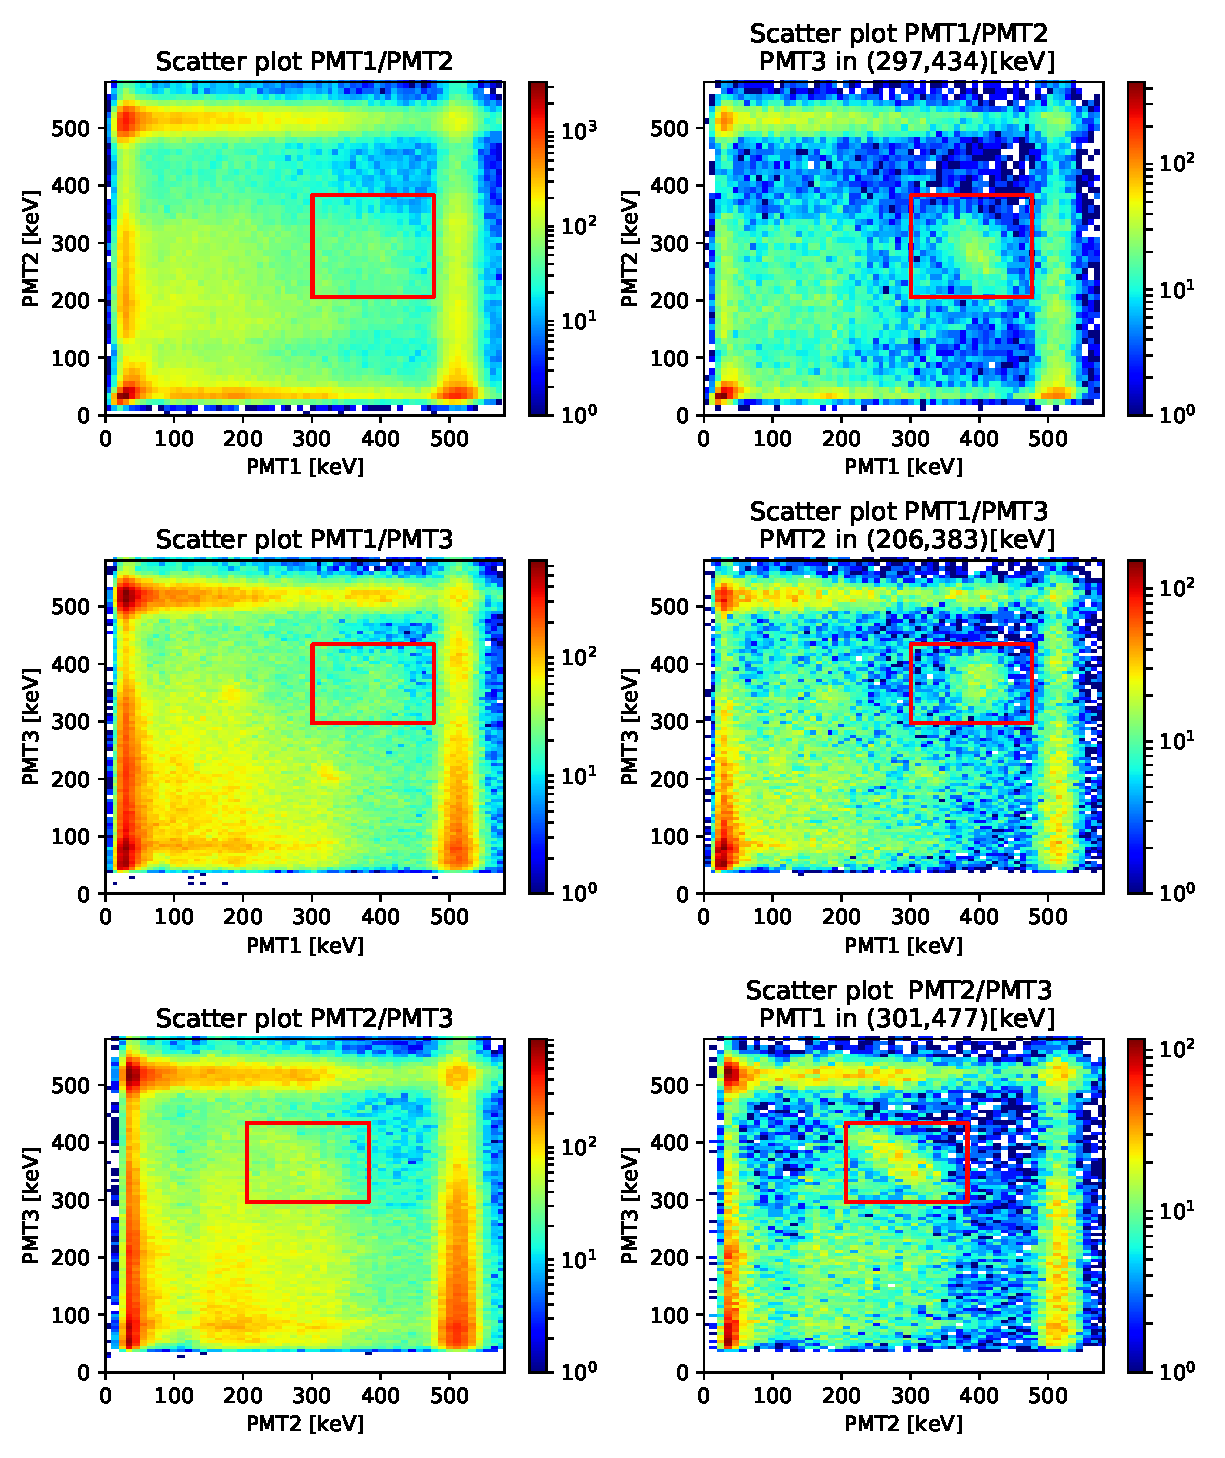
\includegraphics[width=44em]{immagini/3gamma_signal}
	\caption{\label{fig:3gamma_signal} I dati qui rappresentati sono le coincidenze a 3 di una delle 2 prese dati di segnale. Nella colonna di sinistra sono mostrati gli spettri 2D di ciascuna coppia di rivelatori; nella colonna di destra sono mostrati gli spettri 2D di ciascuna coppia di rivelatori dove sono stati selezionati solo gli eventi con energia nell'altro rivelatore in un certo intervallo centrato sul segnale atteso. I box rossi indicano i limiti degli intervalli su ciascun rivelatore. Il segnale è chiaramente visibile nel box.}
\end{figure}

 \begin{figure}[h]
	\hspace{-4em}
	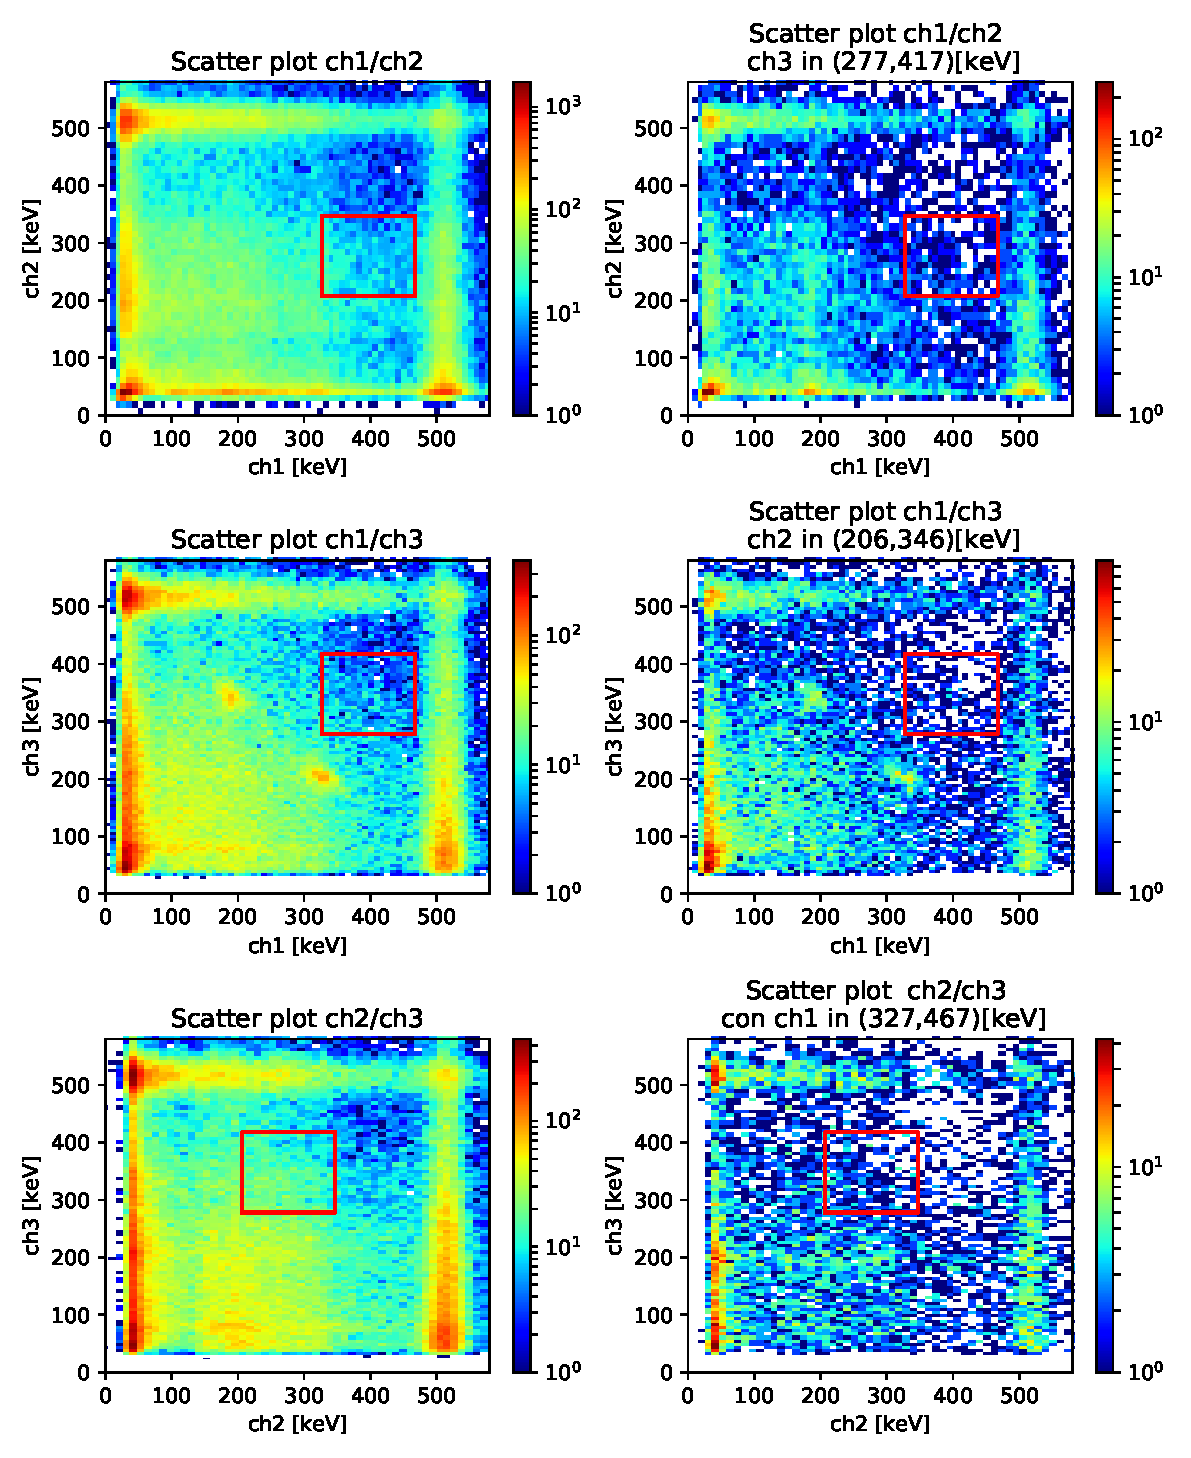
\includegraphics[width=44em]{immagini/3gamma_noise}
	\caption{\label{fig:3gamma_noise} I dati qui rappresentati sono le coincidenze a 3 nella presa dati di rumore. Nella colonna di sinistra sono mostrati gli spettri 2D di ciascuna coppia di rivelatori; nella colonna di destra sono mostrati gli spettri 2D di ciascuna coppia di rivelatori dove sono stati selezionati solo gli eventi con energia nell'altro rivelatore in un certo intervallo centrato sul segnale atteso. I box rossi indicano i limiti degli intervalli su ciascun rivelatore. Nessun segnale è visibile nel box.}
\end{figure}

	

%realizzazione esperimento


%analisi

% Fine

\section{Conclusioni}

La massa dell'elettrone risulta \SI{511(13)}{keV},
compatibile con il valore noto \SI{511}{keV}.
L'incertezza è praticamente solo sistematica e proviene dalla discrepanza tra scintillatori diversi.

Aggiungere i risultati della cattura elettronica e dell'annichilazione a 3$\gamma$.


\begin{thebibliography}{99}

\bibitem[1]{cross}
M.J. Berger, J.H. Hubbell, S.M. Seltzer, J. Chang, J.S. Coursey, R. Sukumar, D.S. Zucker, and K. Olsen, XCOM: Photon Cross Sections Database, \emph{National Institute of Standards and Technology} (2010).

\end{thebibliography}

\end{document}